\documentclass[12pt]{article}

\usepackage[utf8]{inputenc}
\usepackage{amsmath, amssymb, amsfonts, cancel}
\usepackage{graphicx}
\usepackage[letterpaper, left=1in, right=1in, top=1in, bottom=1in]{geometry}
\usepackage{booktabs}
\usepackage{multirow}
\usepackage{float}
\usepackage{caption}
\usepackage{colortbl}
\usepackage{xcolor}
\definecolor{paleYellow}{RGB}{255,255,180}
\usepackage{physics}
\usepackage{hyperref}
\usepackage[spanish]{babel}

\title{
Práctica 5: VLAN, DHCP, ETHERCHANNEL\\[0.5em]
\large Administración de redes
}

\author{
Jorge Alberto Suarez Saldana\\
\small Matrícula: 355992\\
\small Profesor: Raymundo Antonio González Grimaldo
}

\date{\today}

\begin{document}
\maketitle

\section{Topología de la red}
Podemos observar en la Figura \ref{fig:topologia} un diagrama de la topología de la red en el modo lógico del simulador
Cisco Packet Tracer.
\begin{figure}[H]
  \centering
  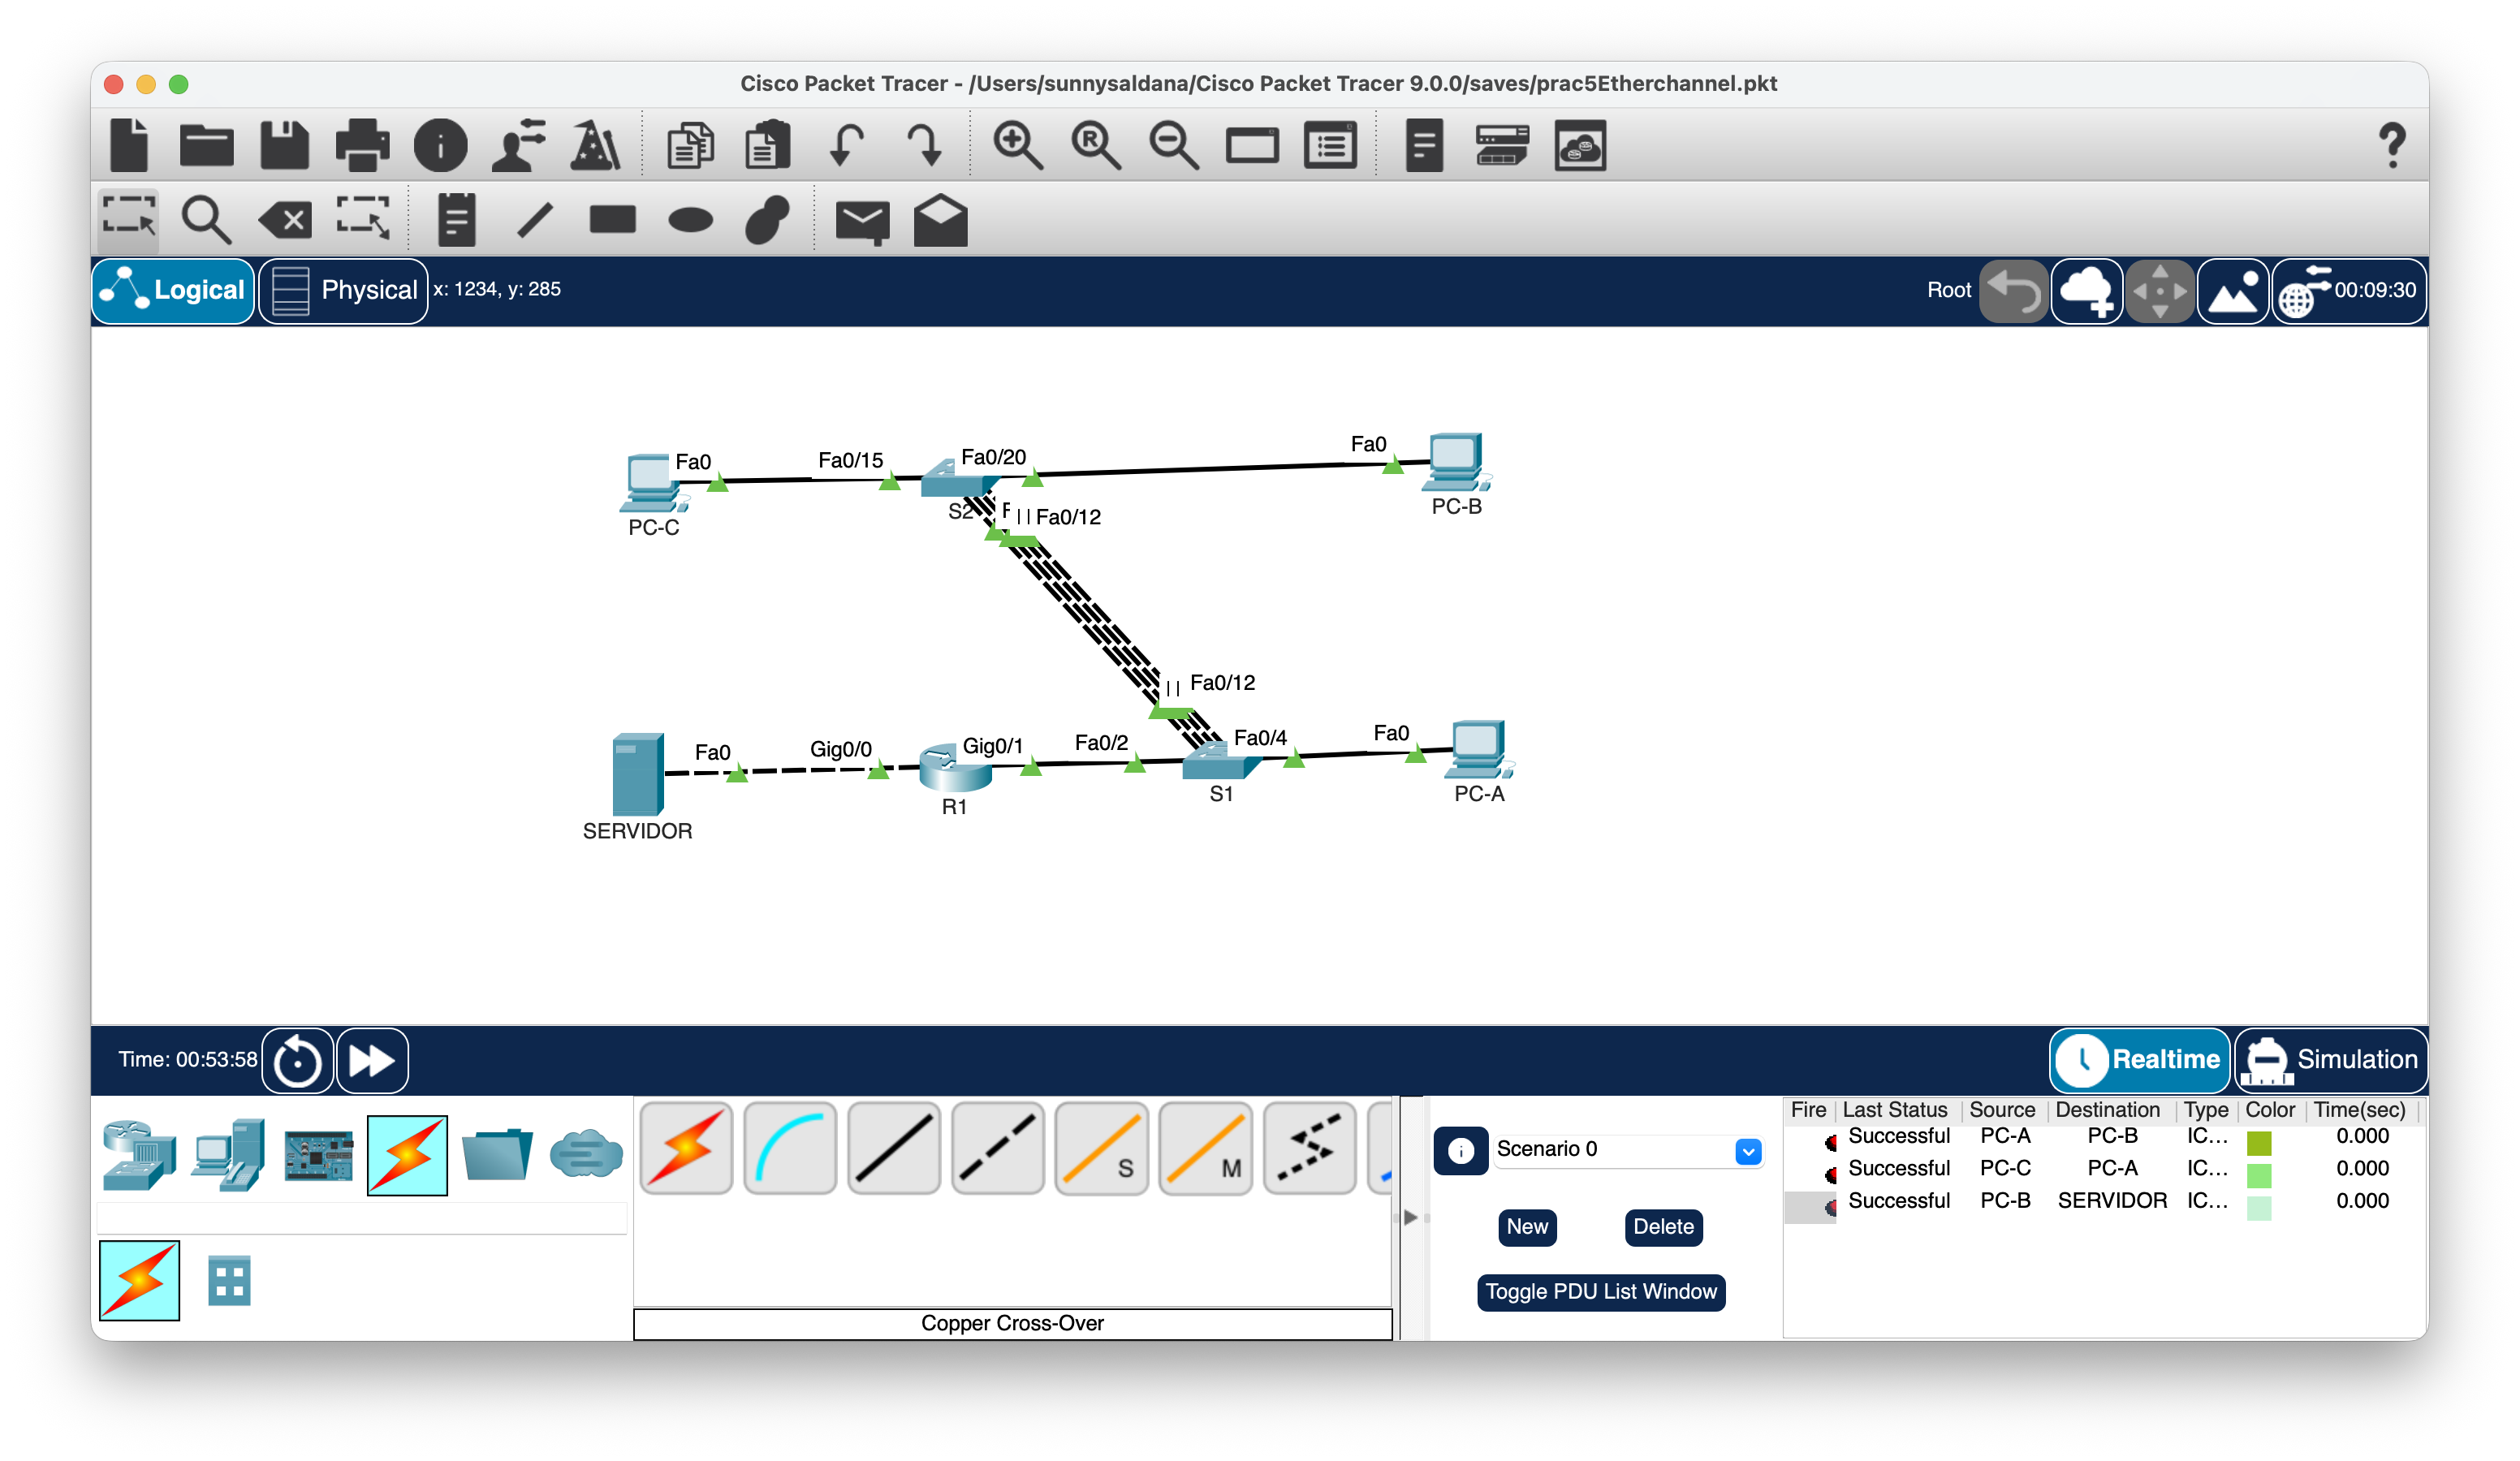
\includegraphics[width=0.8\textwidth]{diagramaTopologia.png}
  \caption{Topología de la red}\label{fig:topologia}
\end{figure}


\section{Tabla de direccionamiento}

\begin{center}
\begin{tabular}{lllll}
\toprule
Dispositivo & Interfaz & Dirección IP & Máscara & Gateway \\
\midrule
R1 & G0/0/0 & 59.9.20.9 & 255.255.255.252 & -- \\
R1 & G0/0/1.49 & 186.72.49.1 & 255.255.255.0 & -- \\
R1 & G0/0/1.30 & 186.72.30.1 & 255.255.255.0 & -- \\
R1 & G0/0/1.79 & 186.72.79.1 & 255.255.255.0 & -- \\
R1 & G0/0/1.98 & 186.72.98.1 & 255.255.255.0 & -- \\
S1 & VLAN 98 & 186.72.98.2 & 255.255.255.0 & 186.72.98.1 \\
S2 & VLAN 98 & 186.72.98.3 & 255.255.255.0 & 186.72.98.1 \\
PC-A & NIC & DHCP & 255.255.255.0 & 186.72.79.1 \\
PC-B & NIC & DHCP & 255.255.255.0 & 186.72.30.1 \\
PC-C & NIC & DHCP & 255.255.255.0 & 186.72.49.1 \\
SERVER & NIC & 59.9.20.10 & 255.255.255.252 & 59.9.20.9 \\
\bottomrule
\end{tabular}
\end{center}

\section{Configuración activa de los dispositivos}
Ejecutamos el comando \textit{show running-config} en R1, S1 y S2 para que nos muestren 
su configuración activa.

\subsection{R1}
\begin{figure}[H]
  \centering
  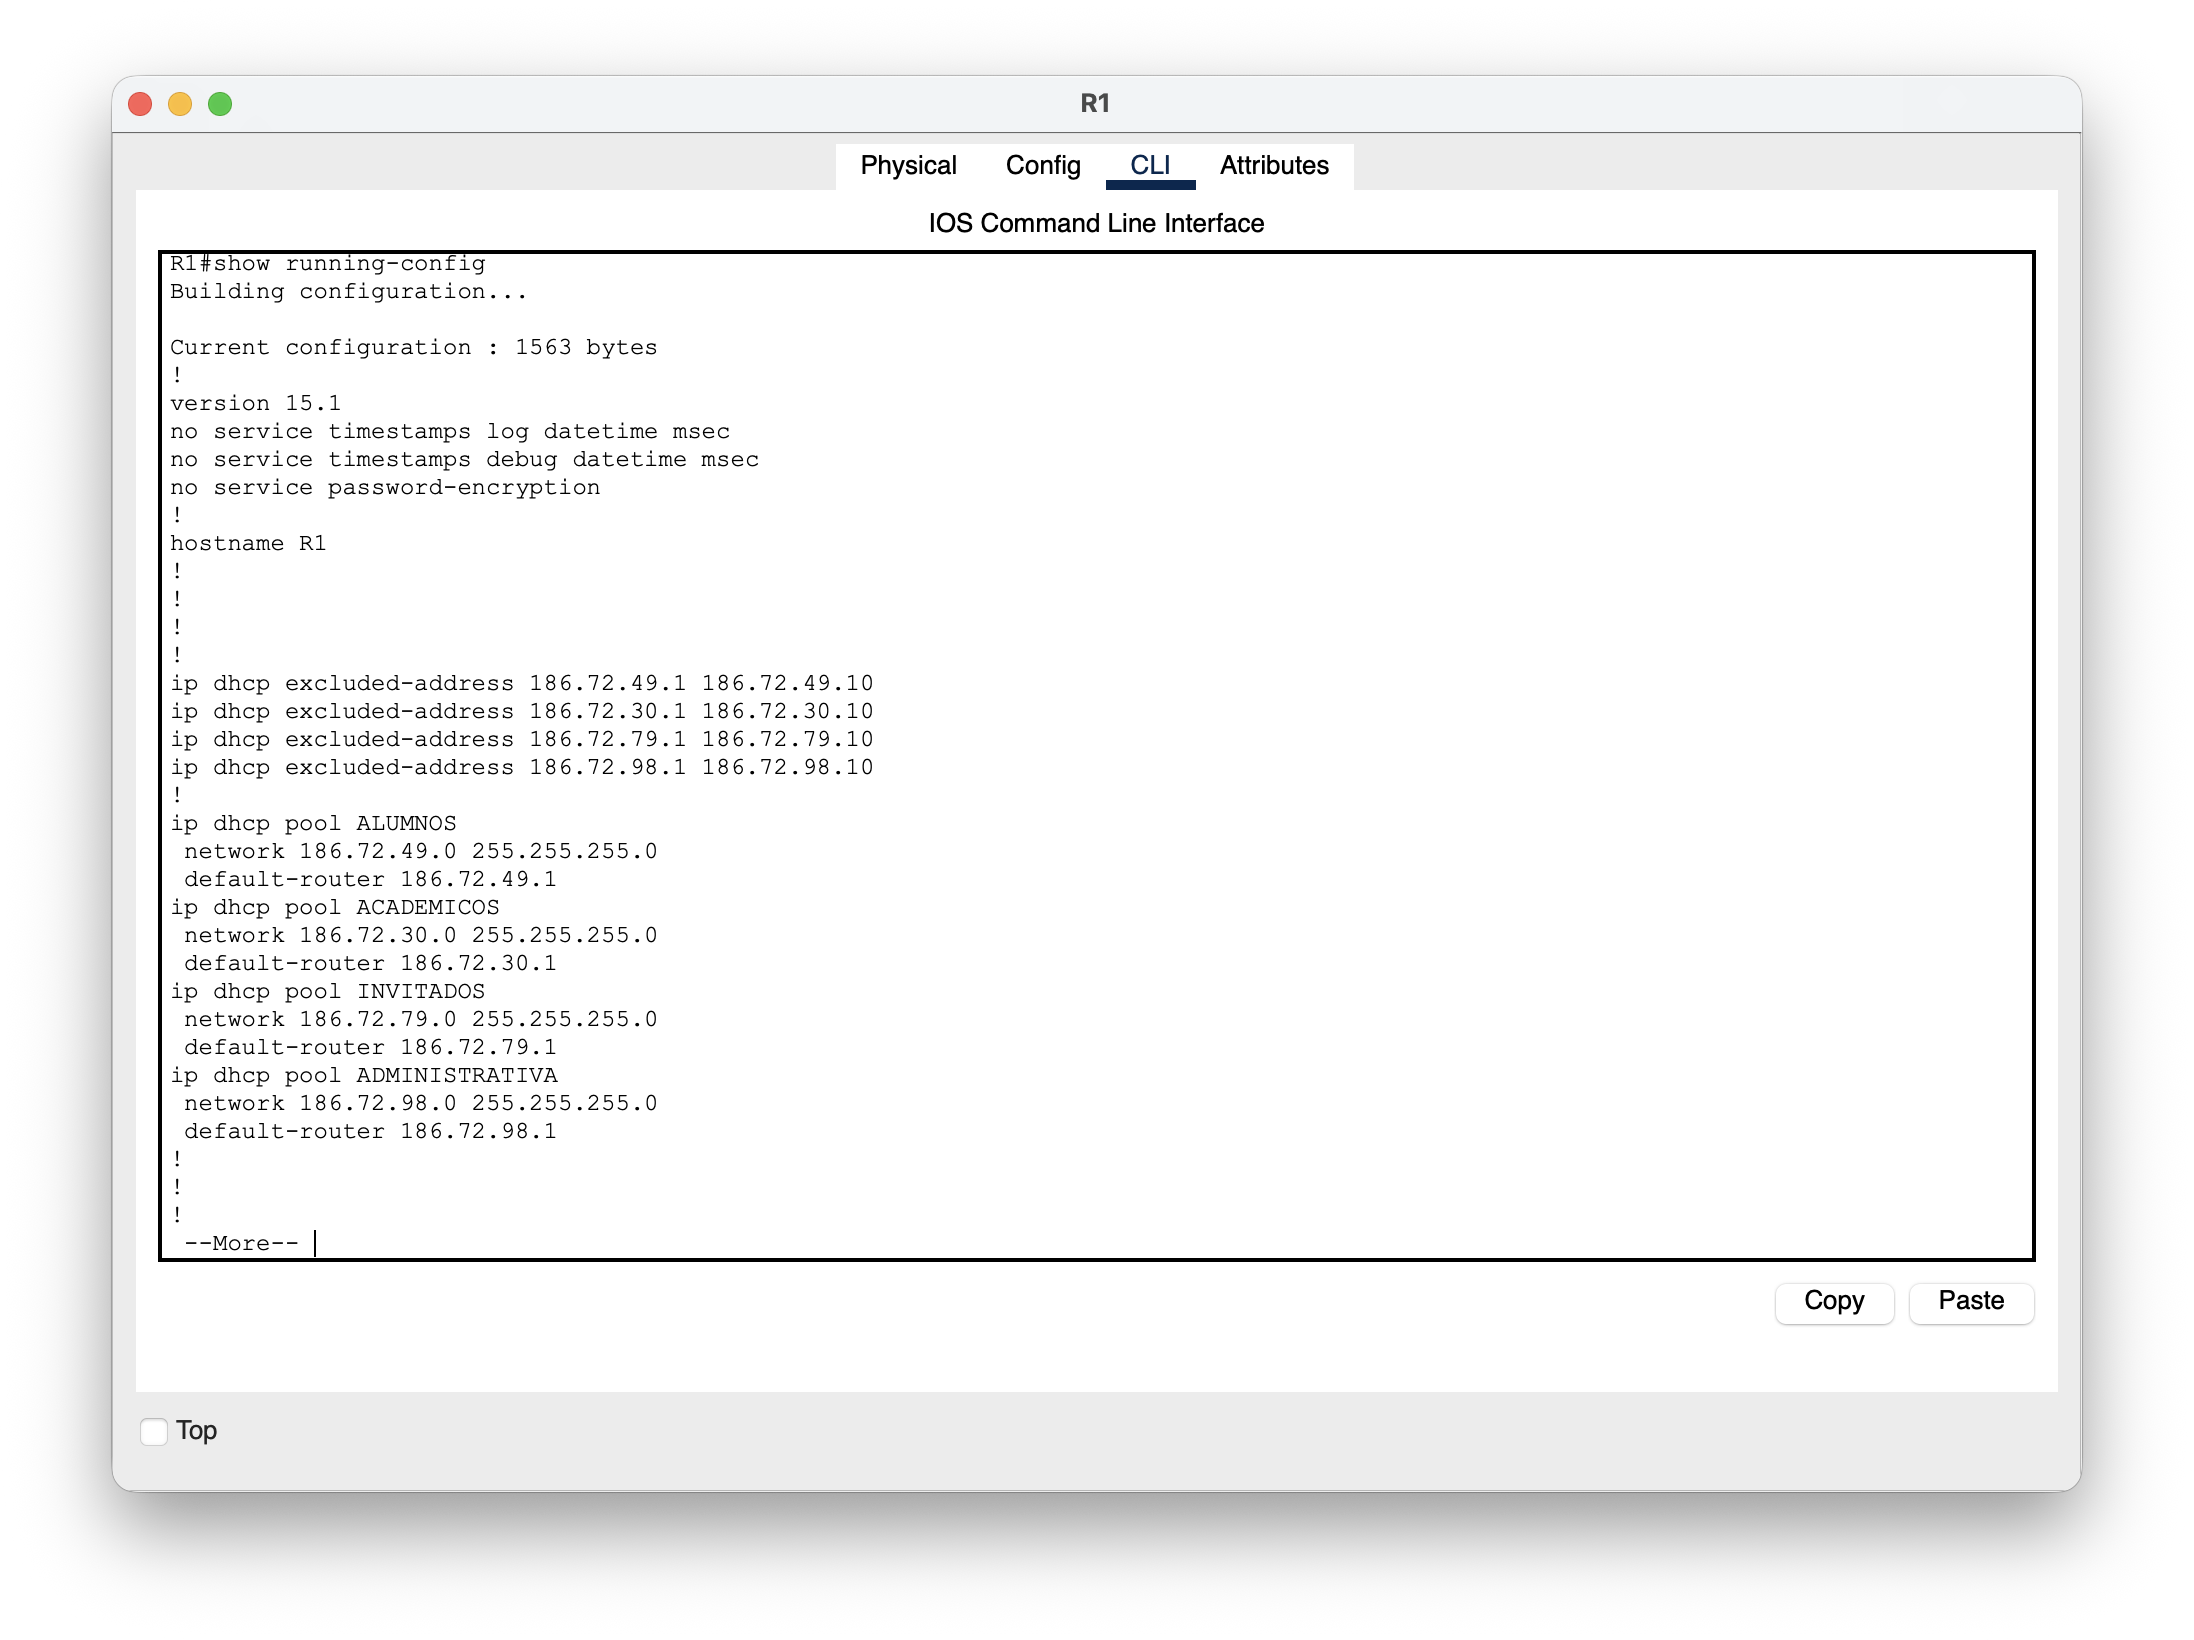
\includegraphics[width=0.8\textwidth]{running-configR1.png}
  \caption{Configuración activa R1}\label{fig:running-configR1}
\end{figure}


\begin{figure}[H]
  \centering
  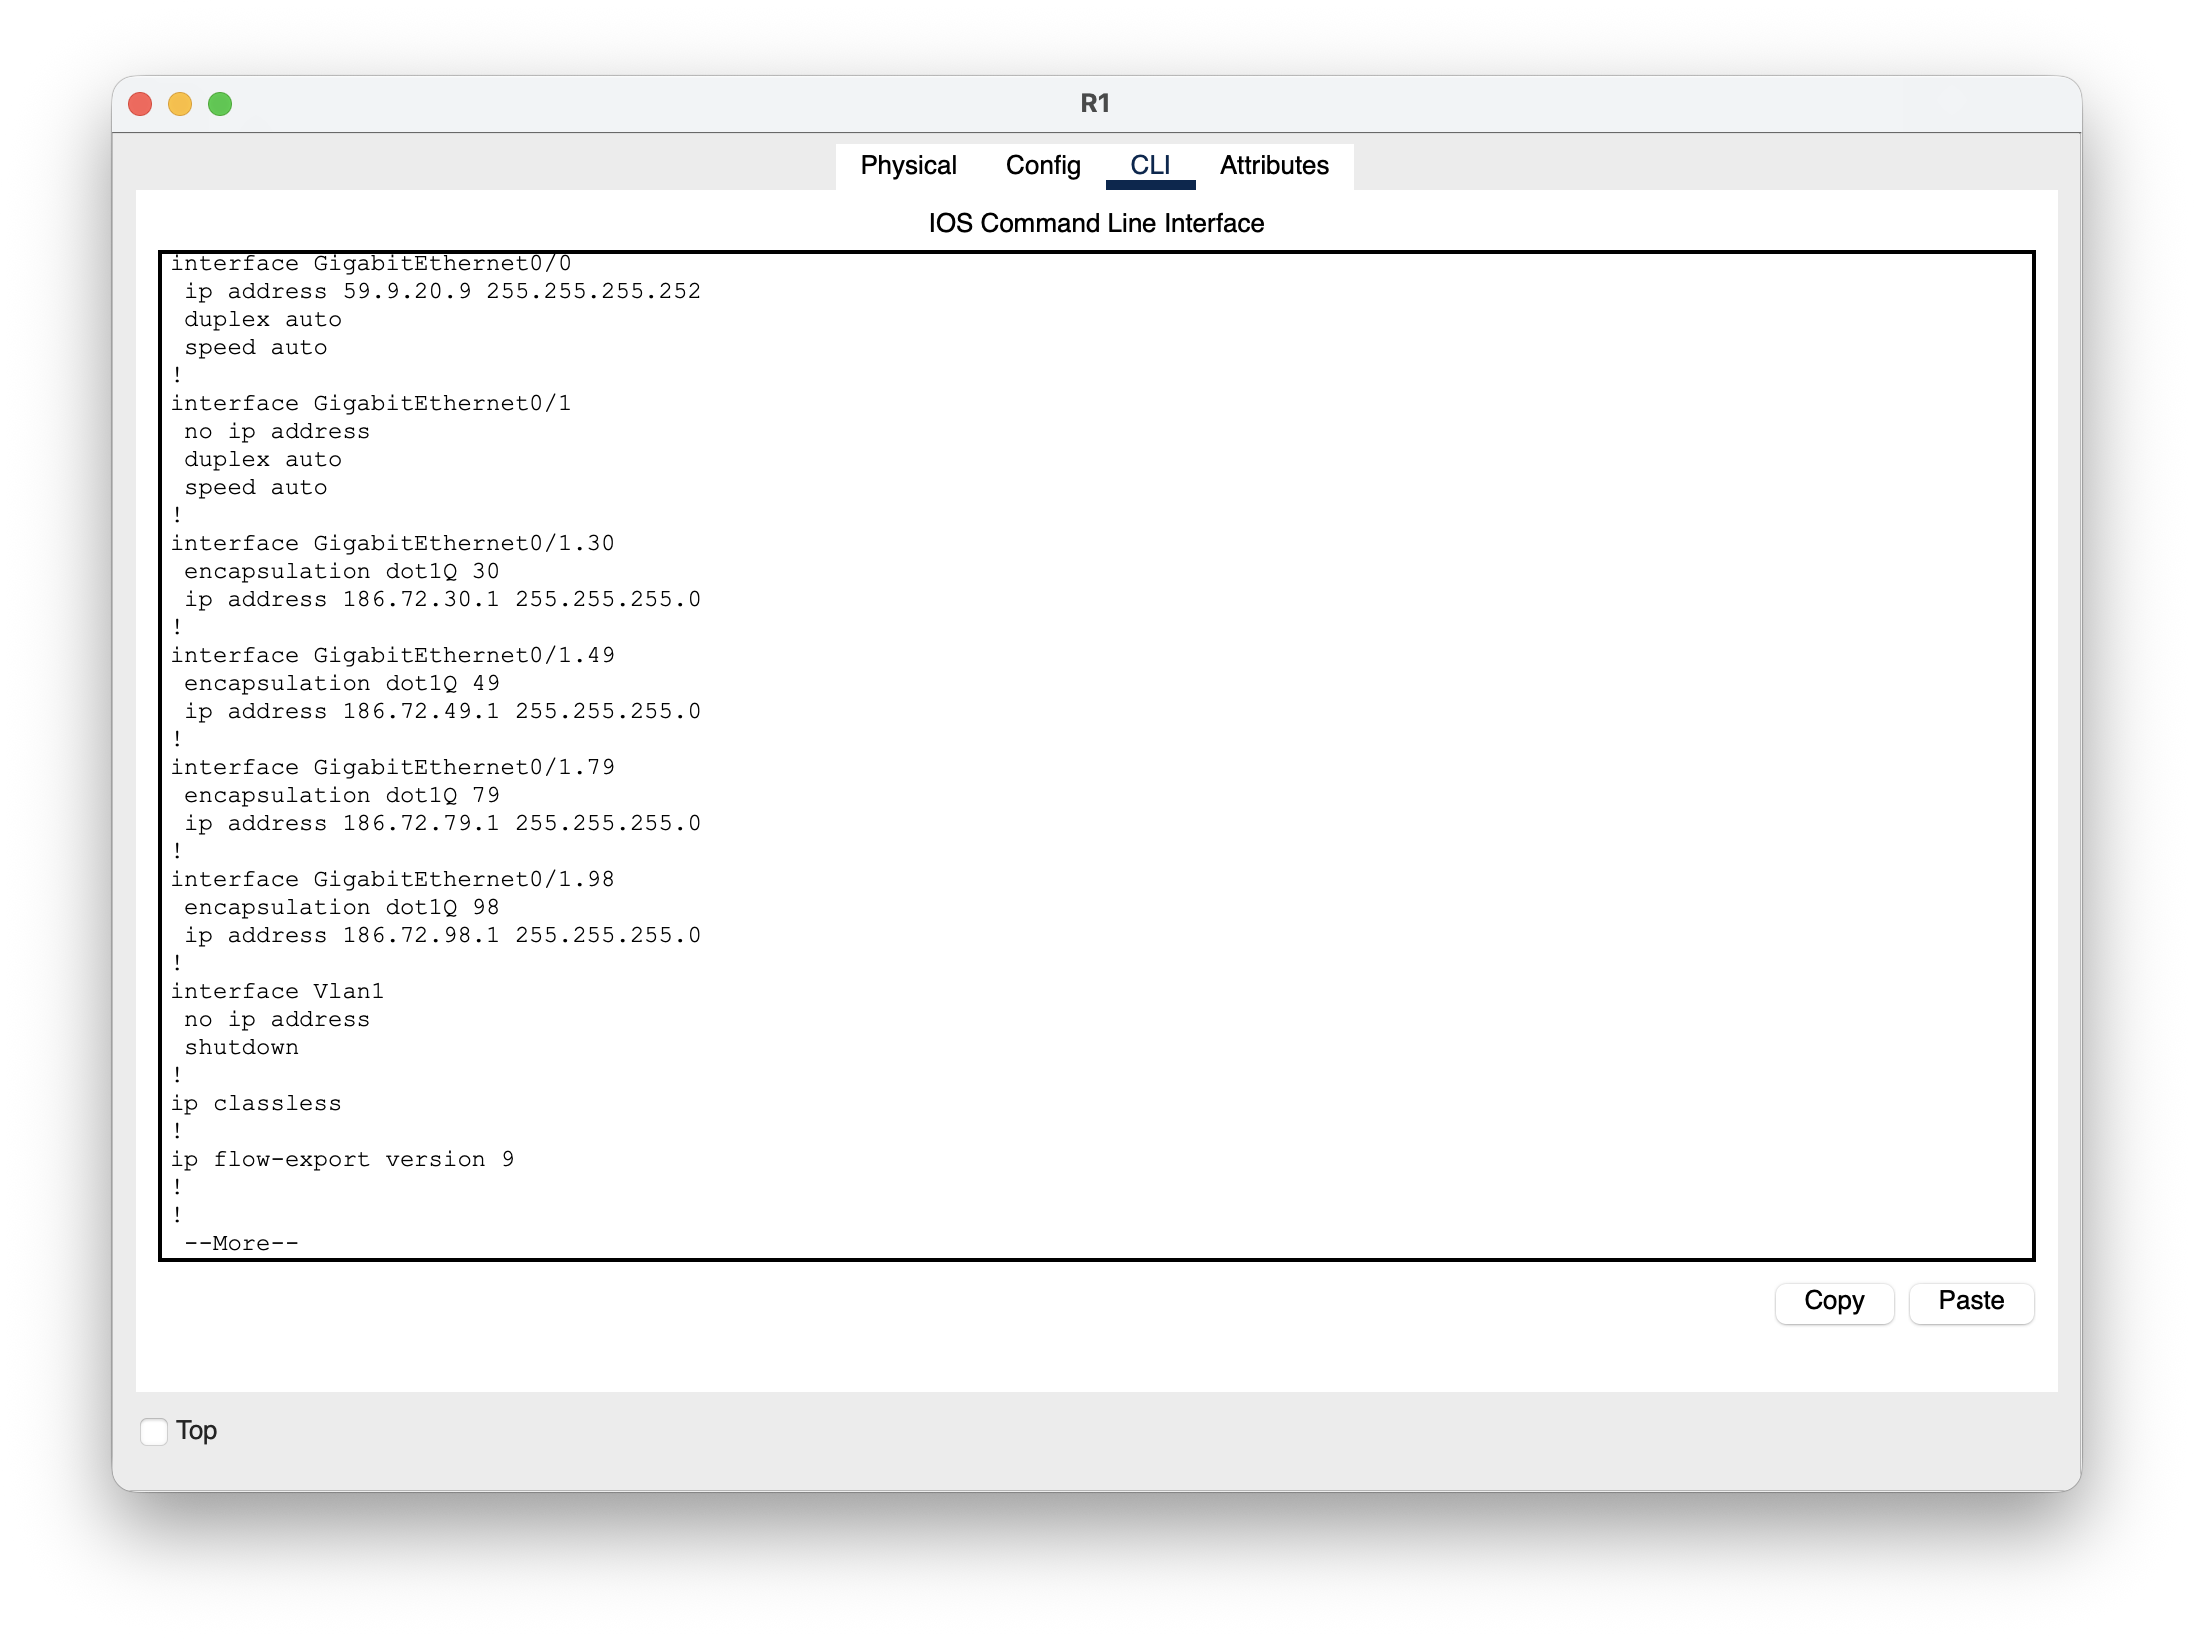
\includegraphics[width=0.8\textwidth]{running-configR1(2).png}
  \caption{Configuración activa R1 (continuación)}\label{fig:running-configR1(2)}
\end{figure}

\subsection{S1}
\begin{figure}[H]
  \centering
  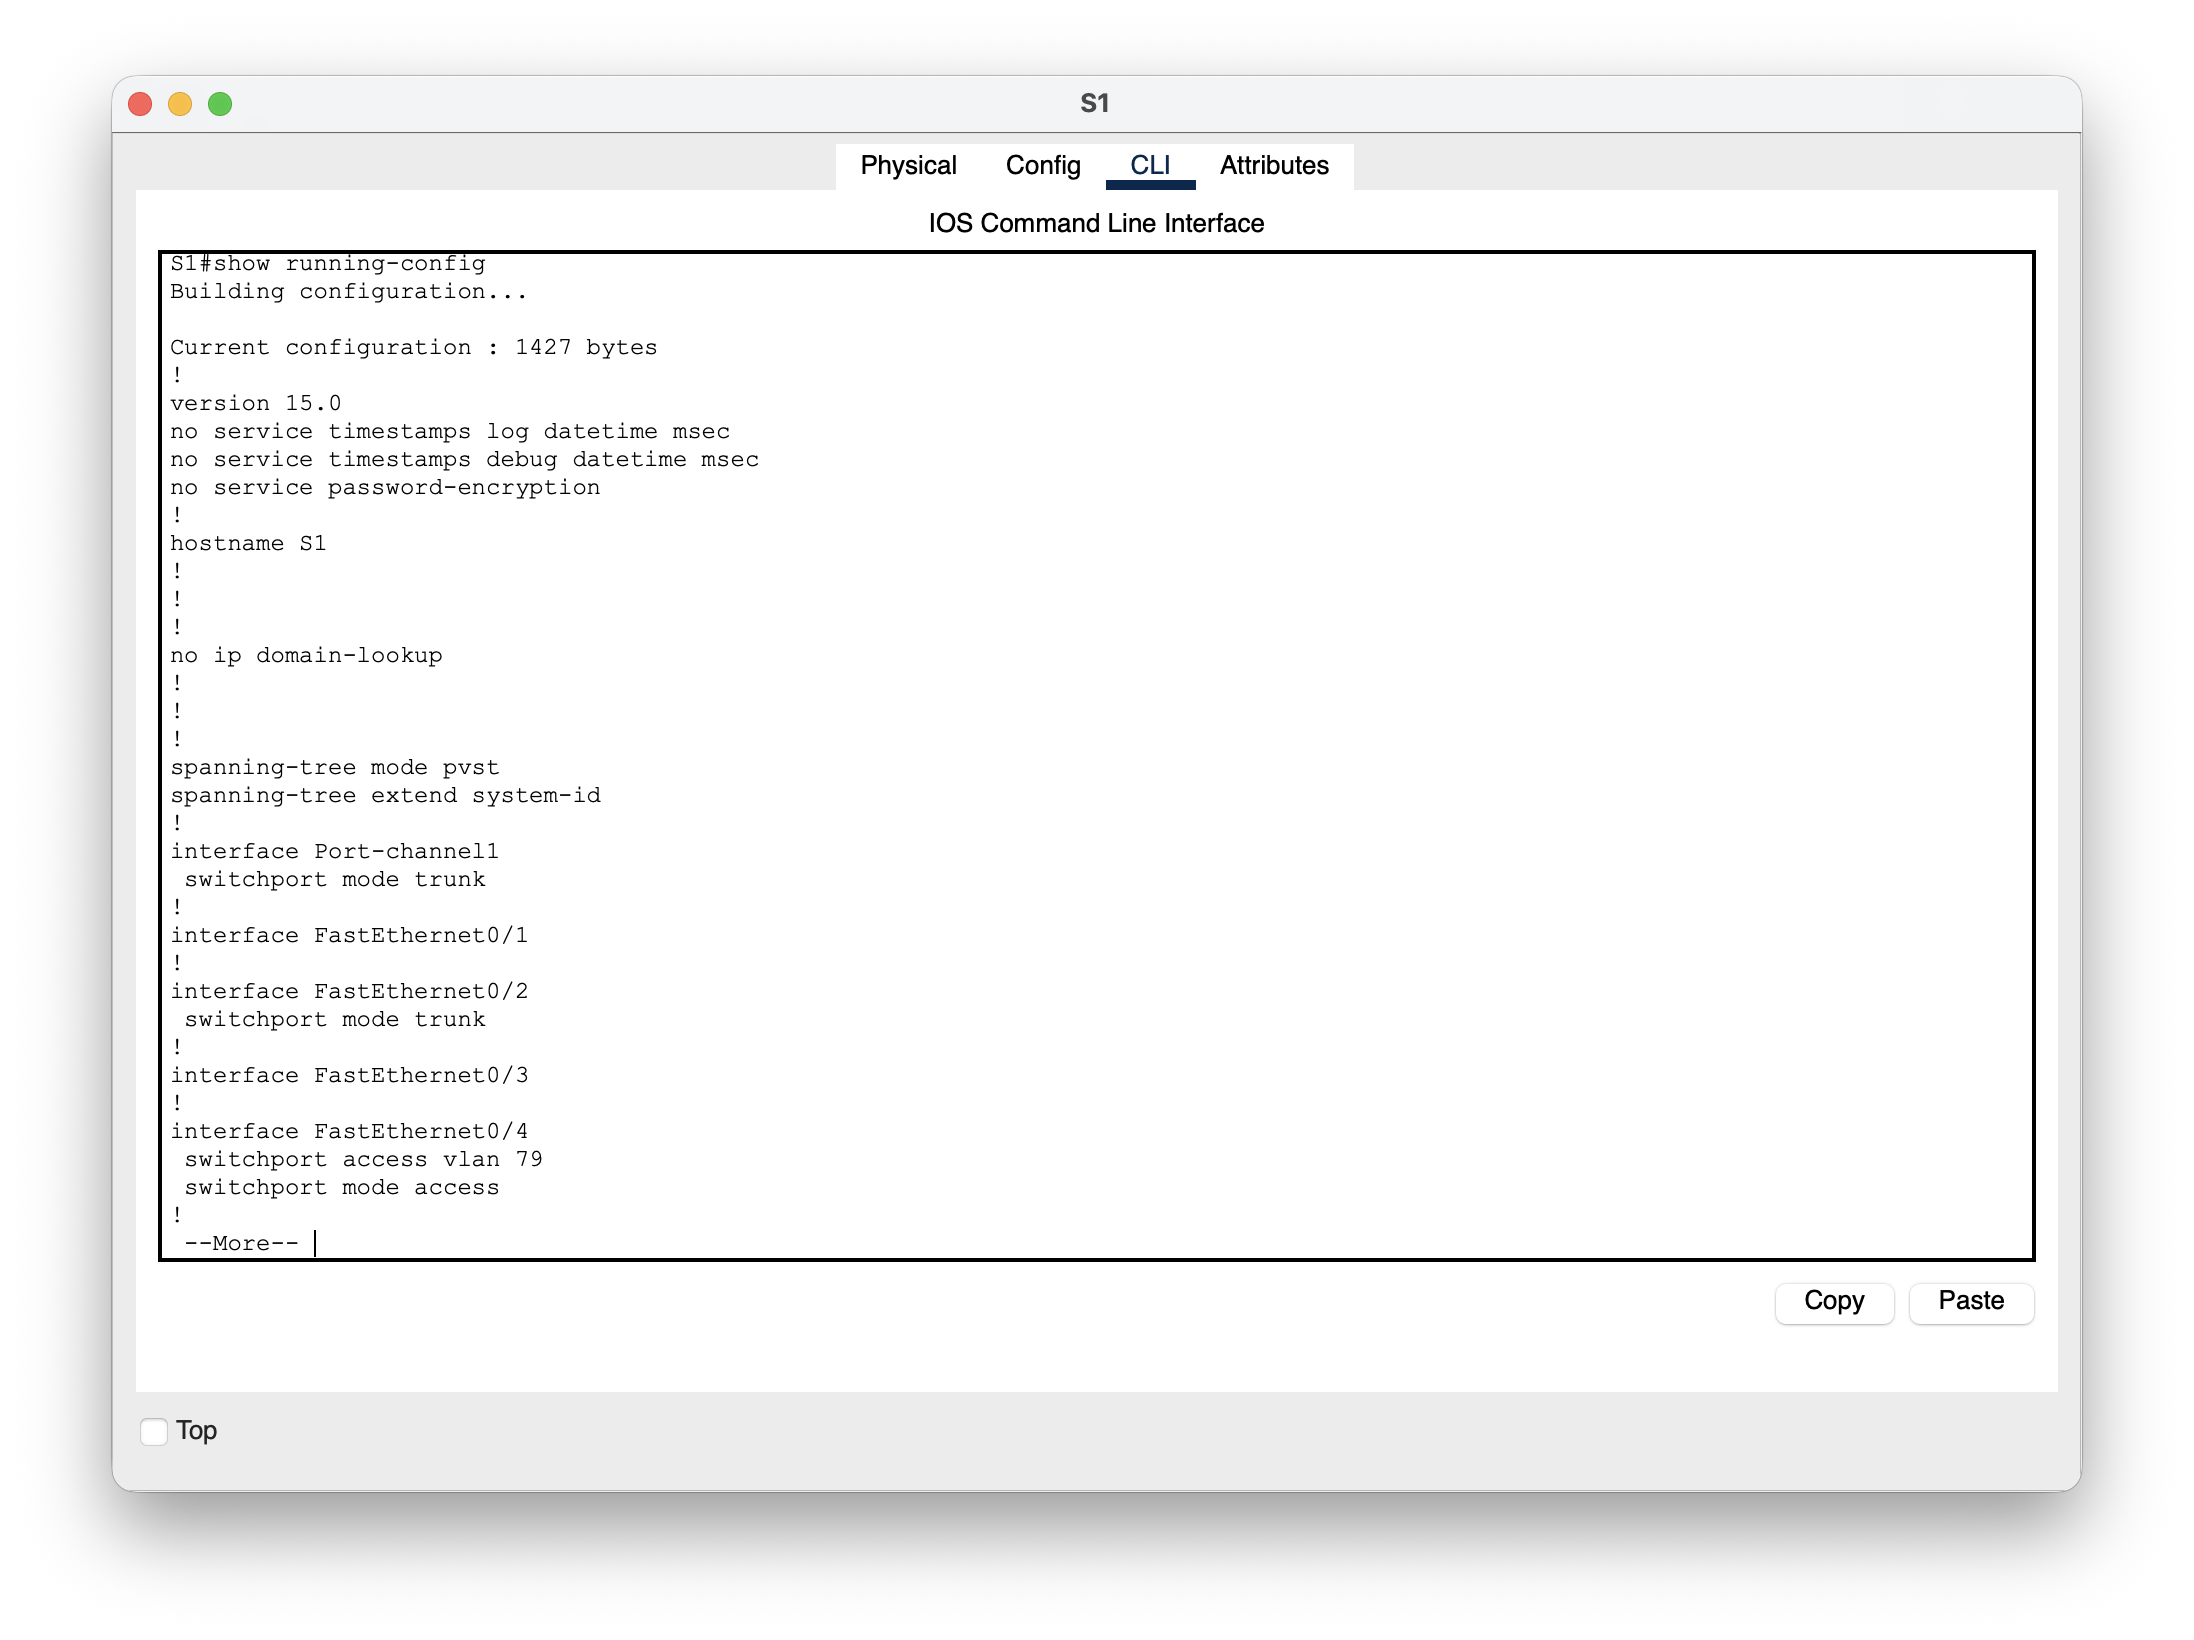
\includegraphics[width=0.8\textwidth]{running-configS1.png}
  \caption{Configuración activa S1}\label{fig:running-configS1}
\end{figure}


\begin{figure}[H]
  \centering
  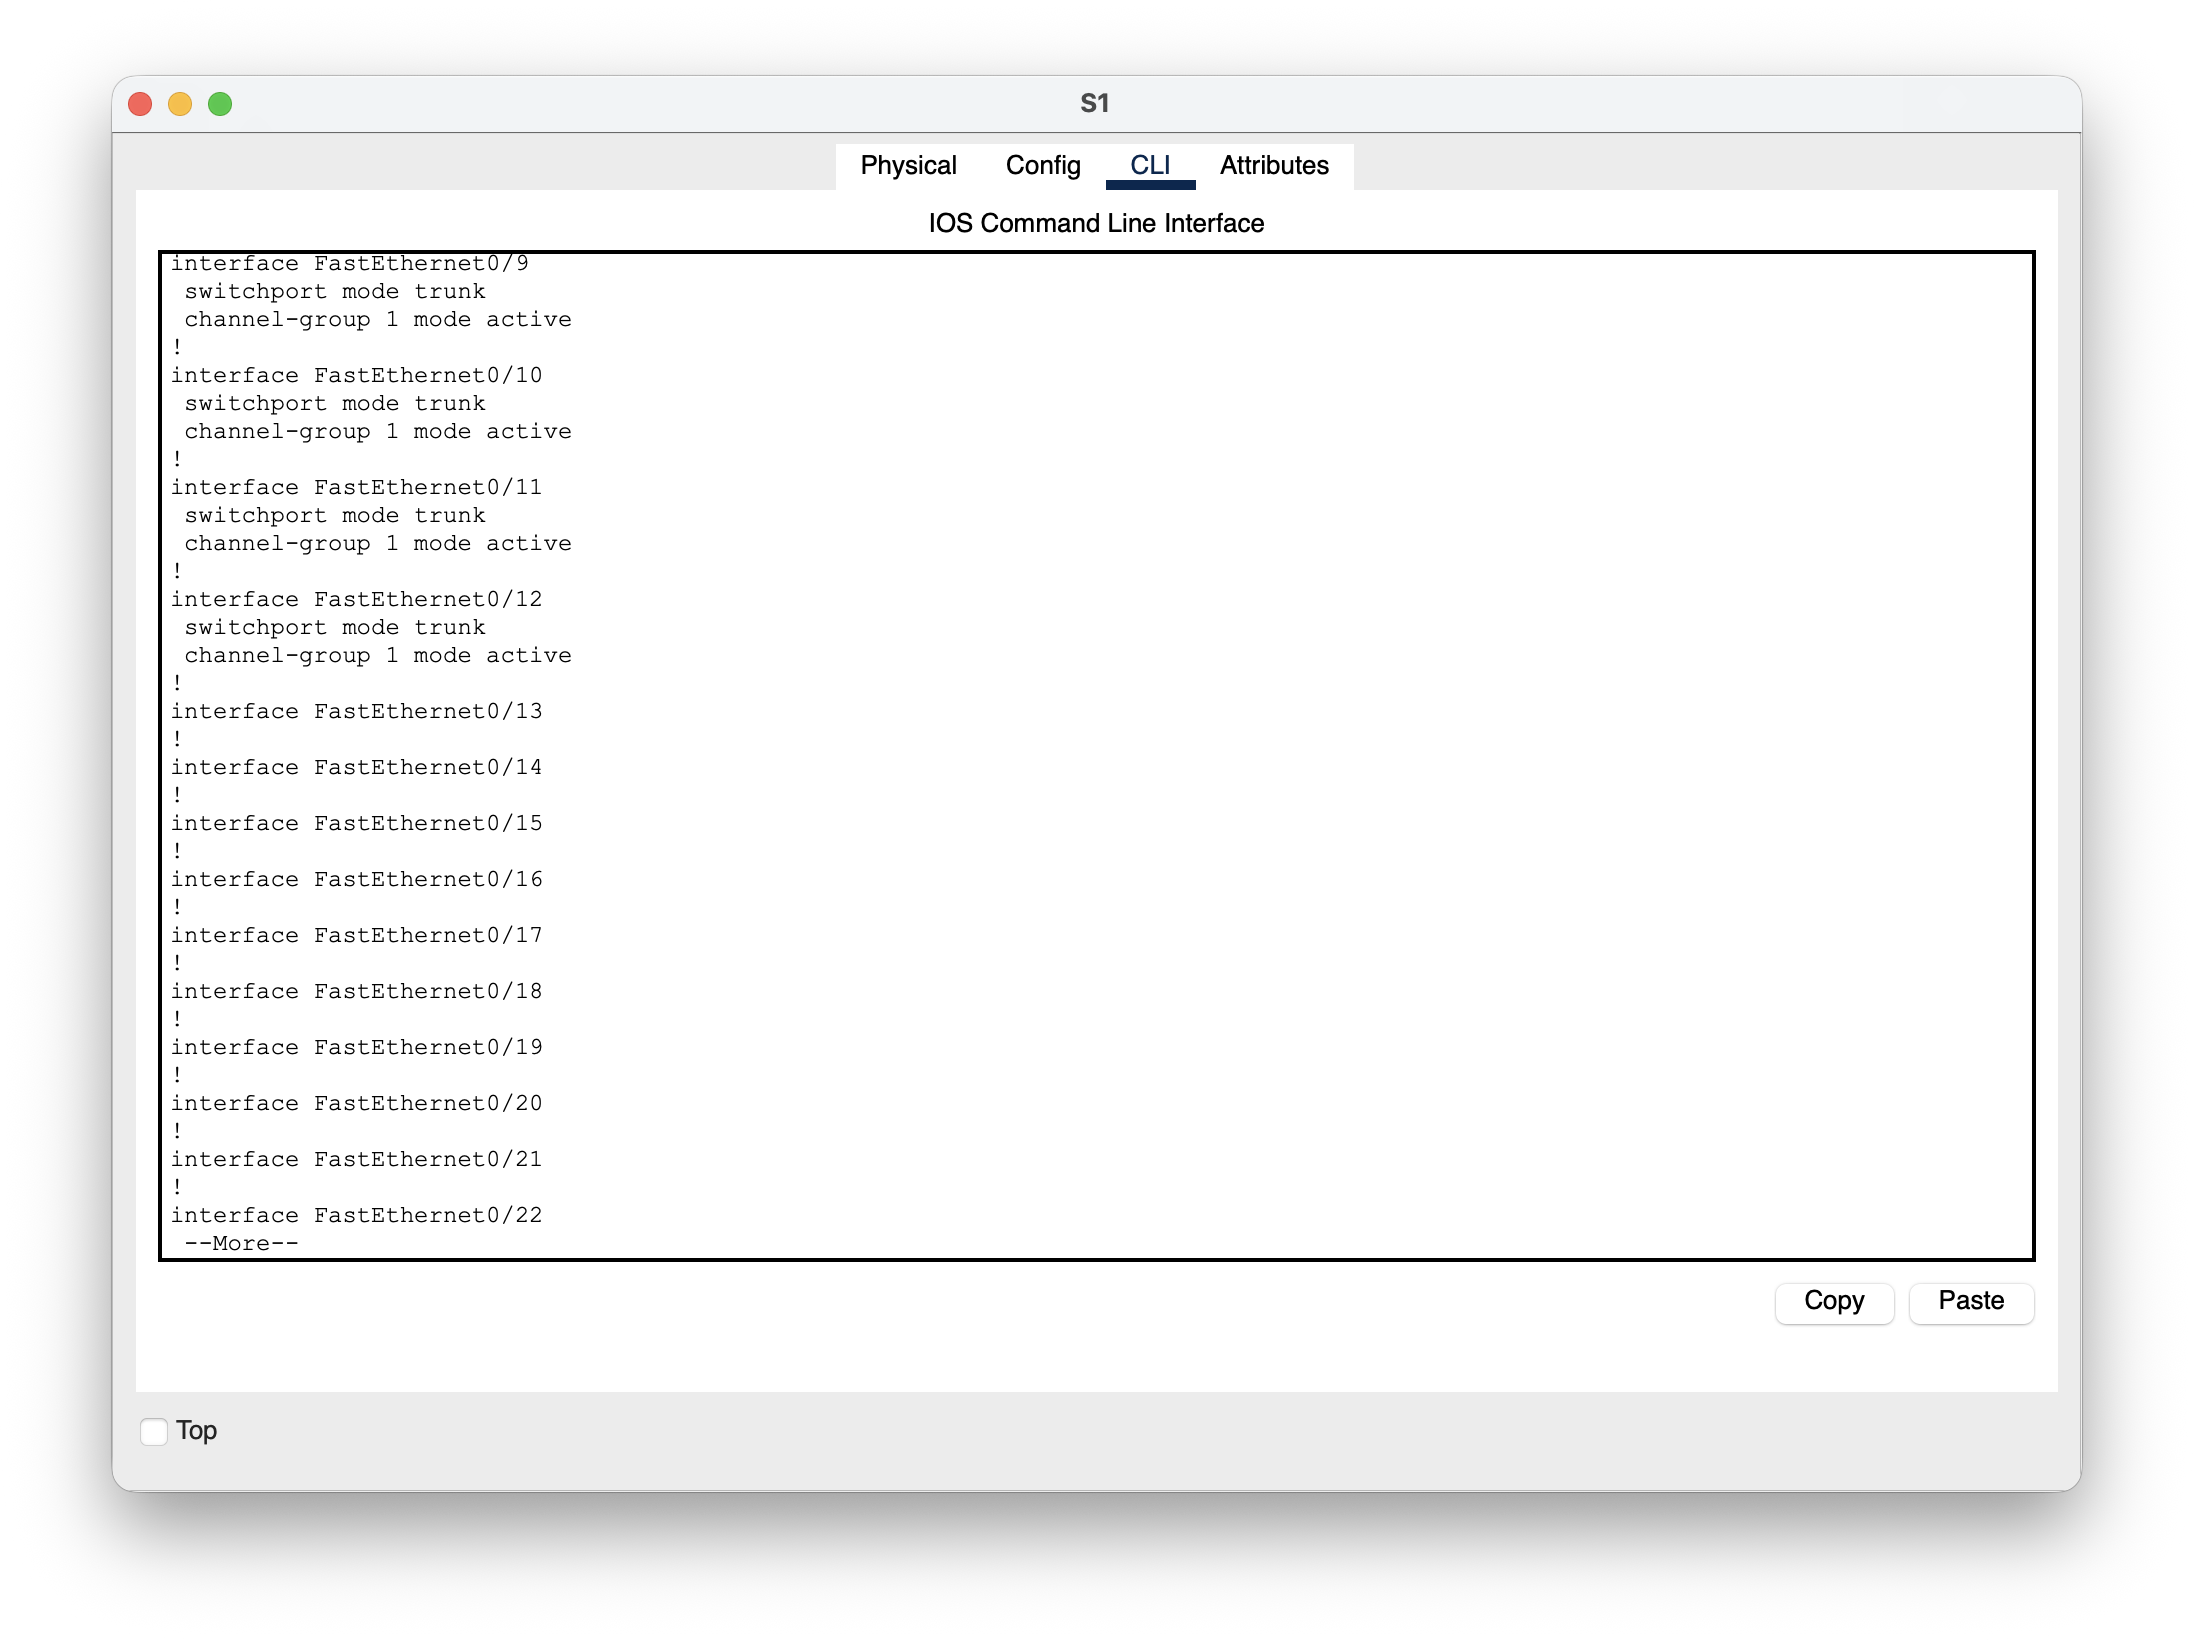
\includegraphics[width=0.8\textwidth]{running-configS1(2).png}
  \caption{Configuración activa S1 (continuación)}\label{fig:running-configS1(2)}
\end{figure}

\subsection{S2}
\begin{figure}[H]
  \centering
  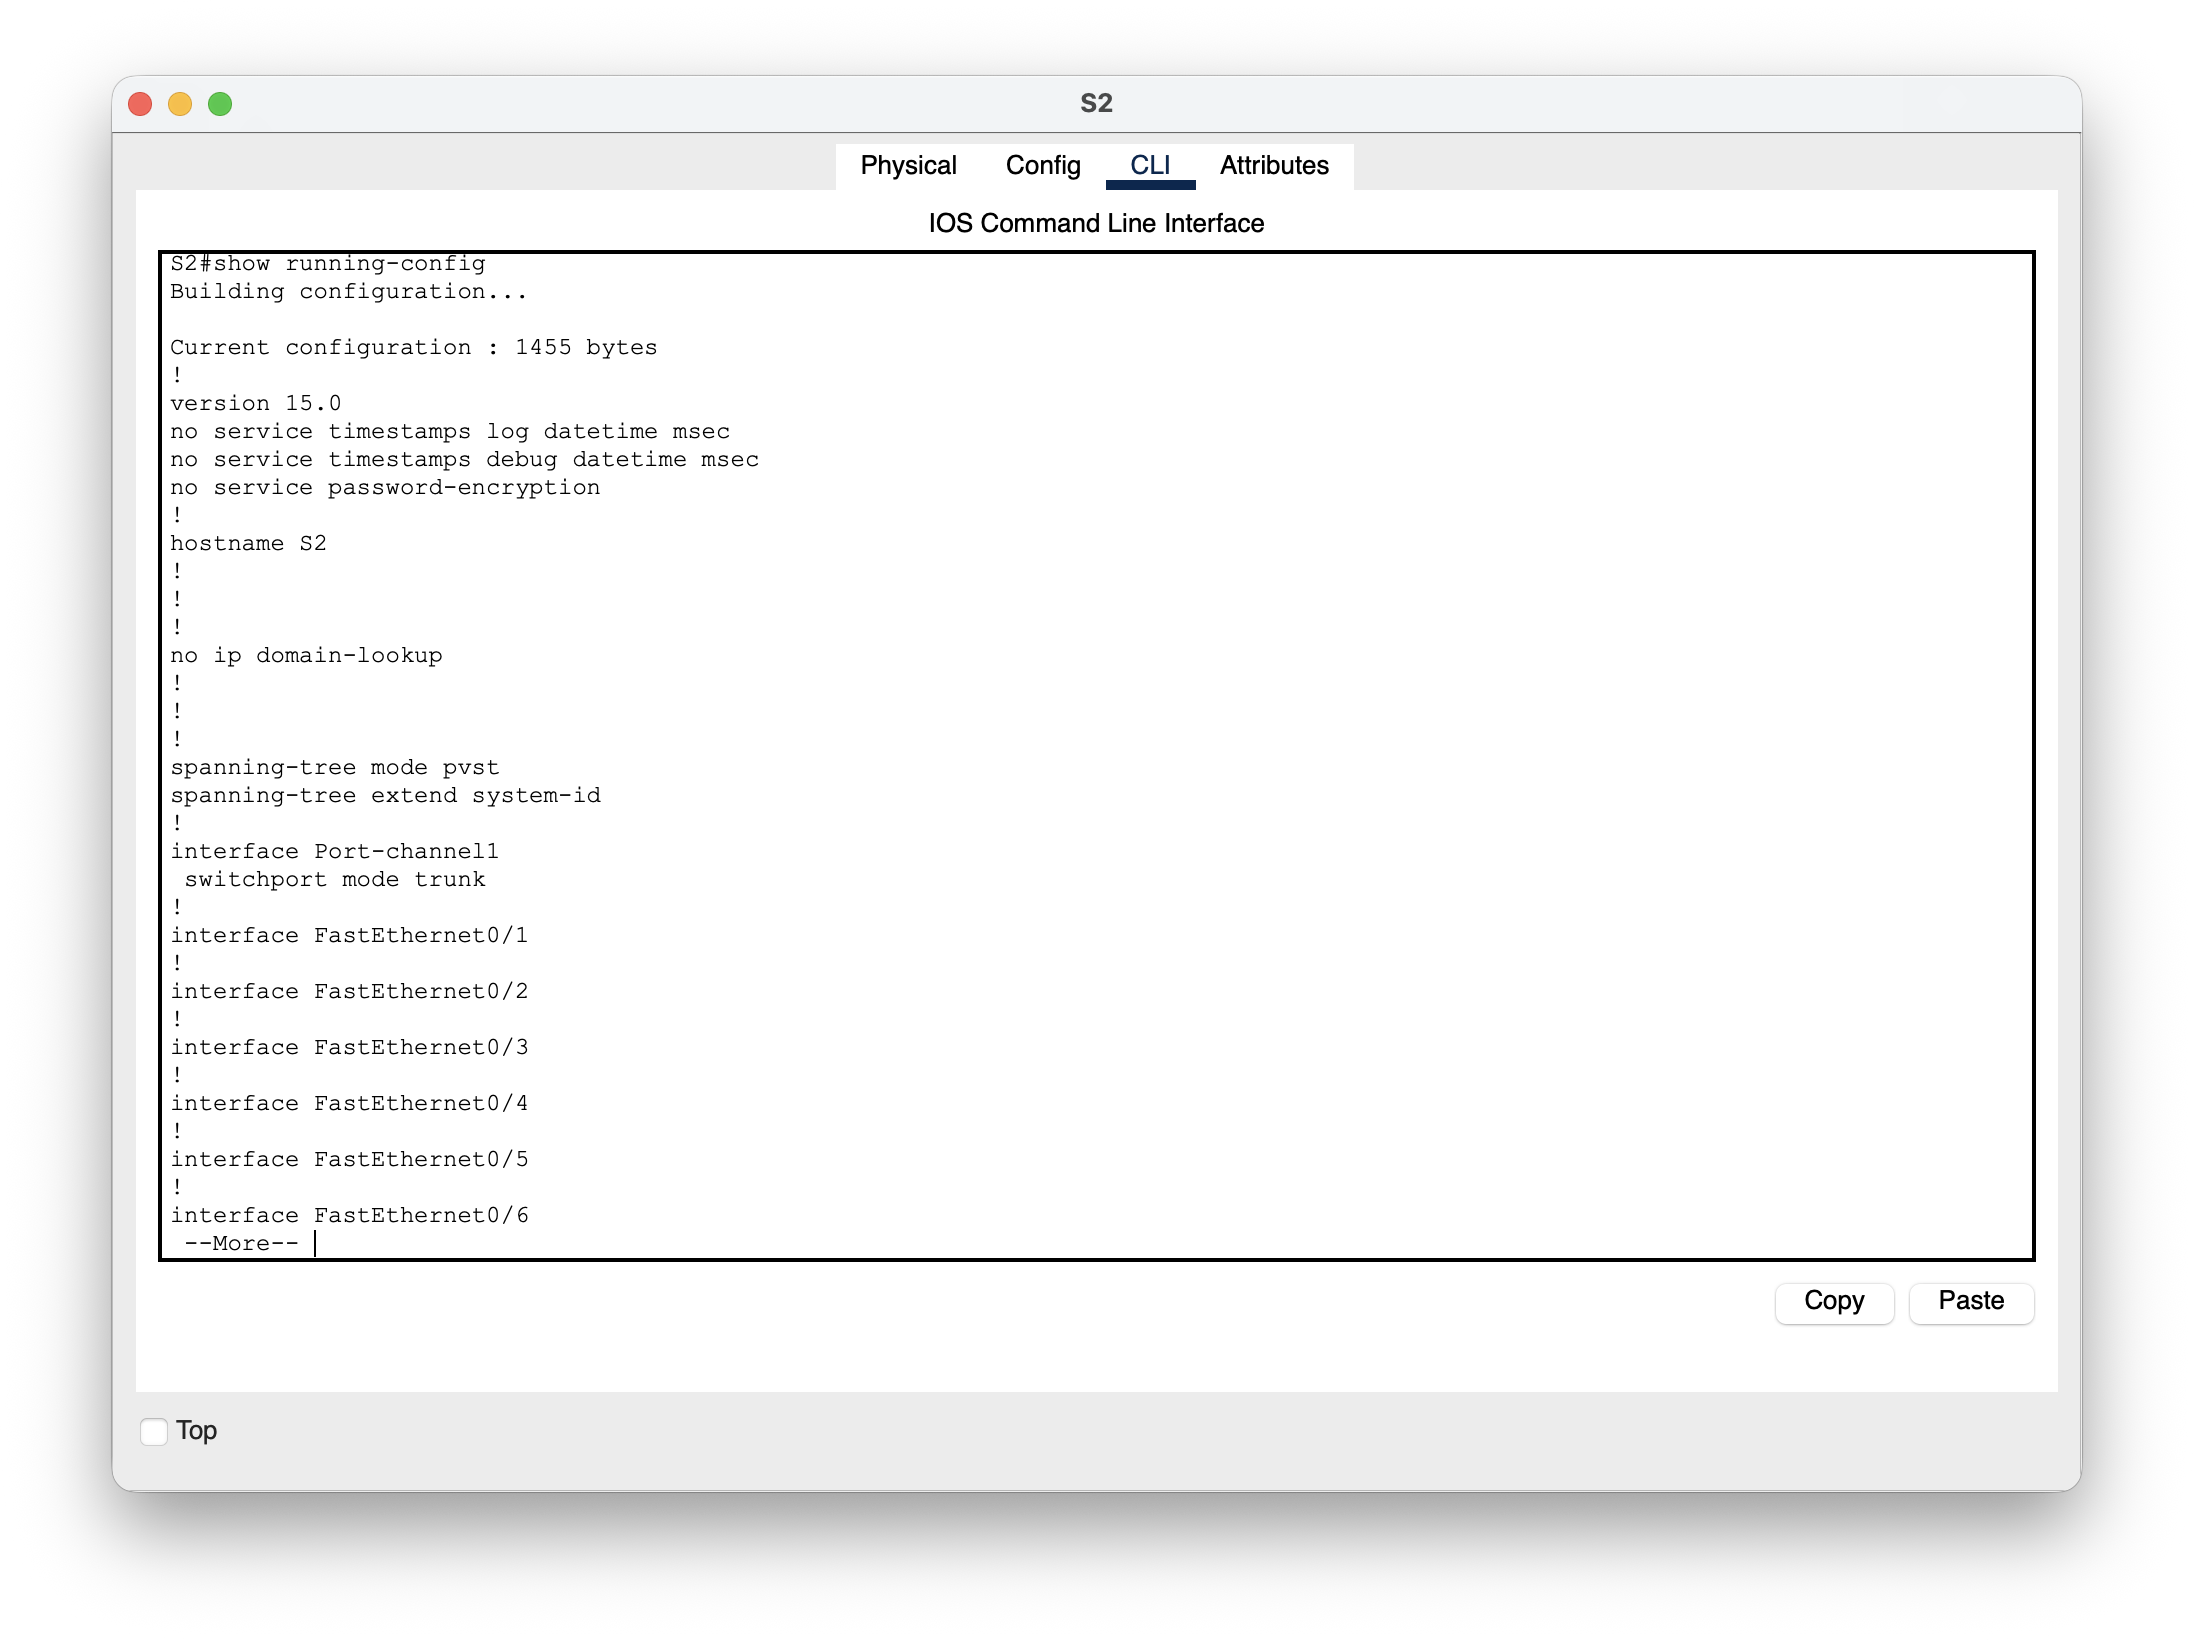
\includegraphics[width=0.8\textwidth]{running-configS2.png}
  \caption{Configuración activa S2}\label{fig:running-configS2}
\end{figure}


\begin{figure}[H]
  \centering
  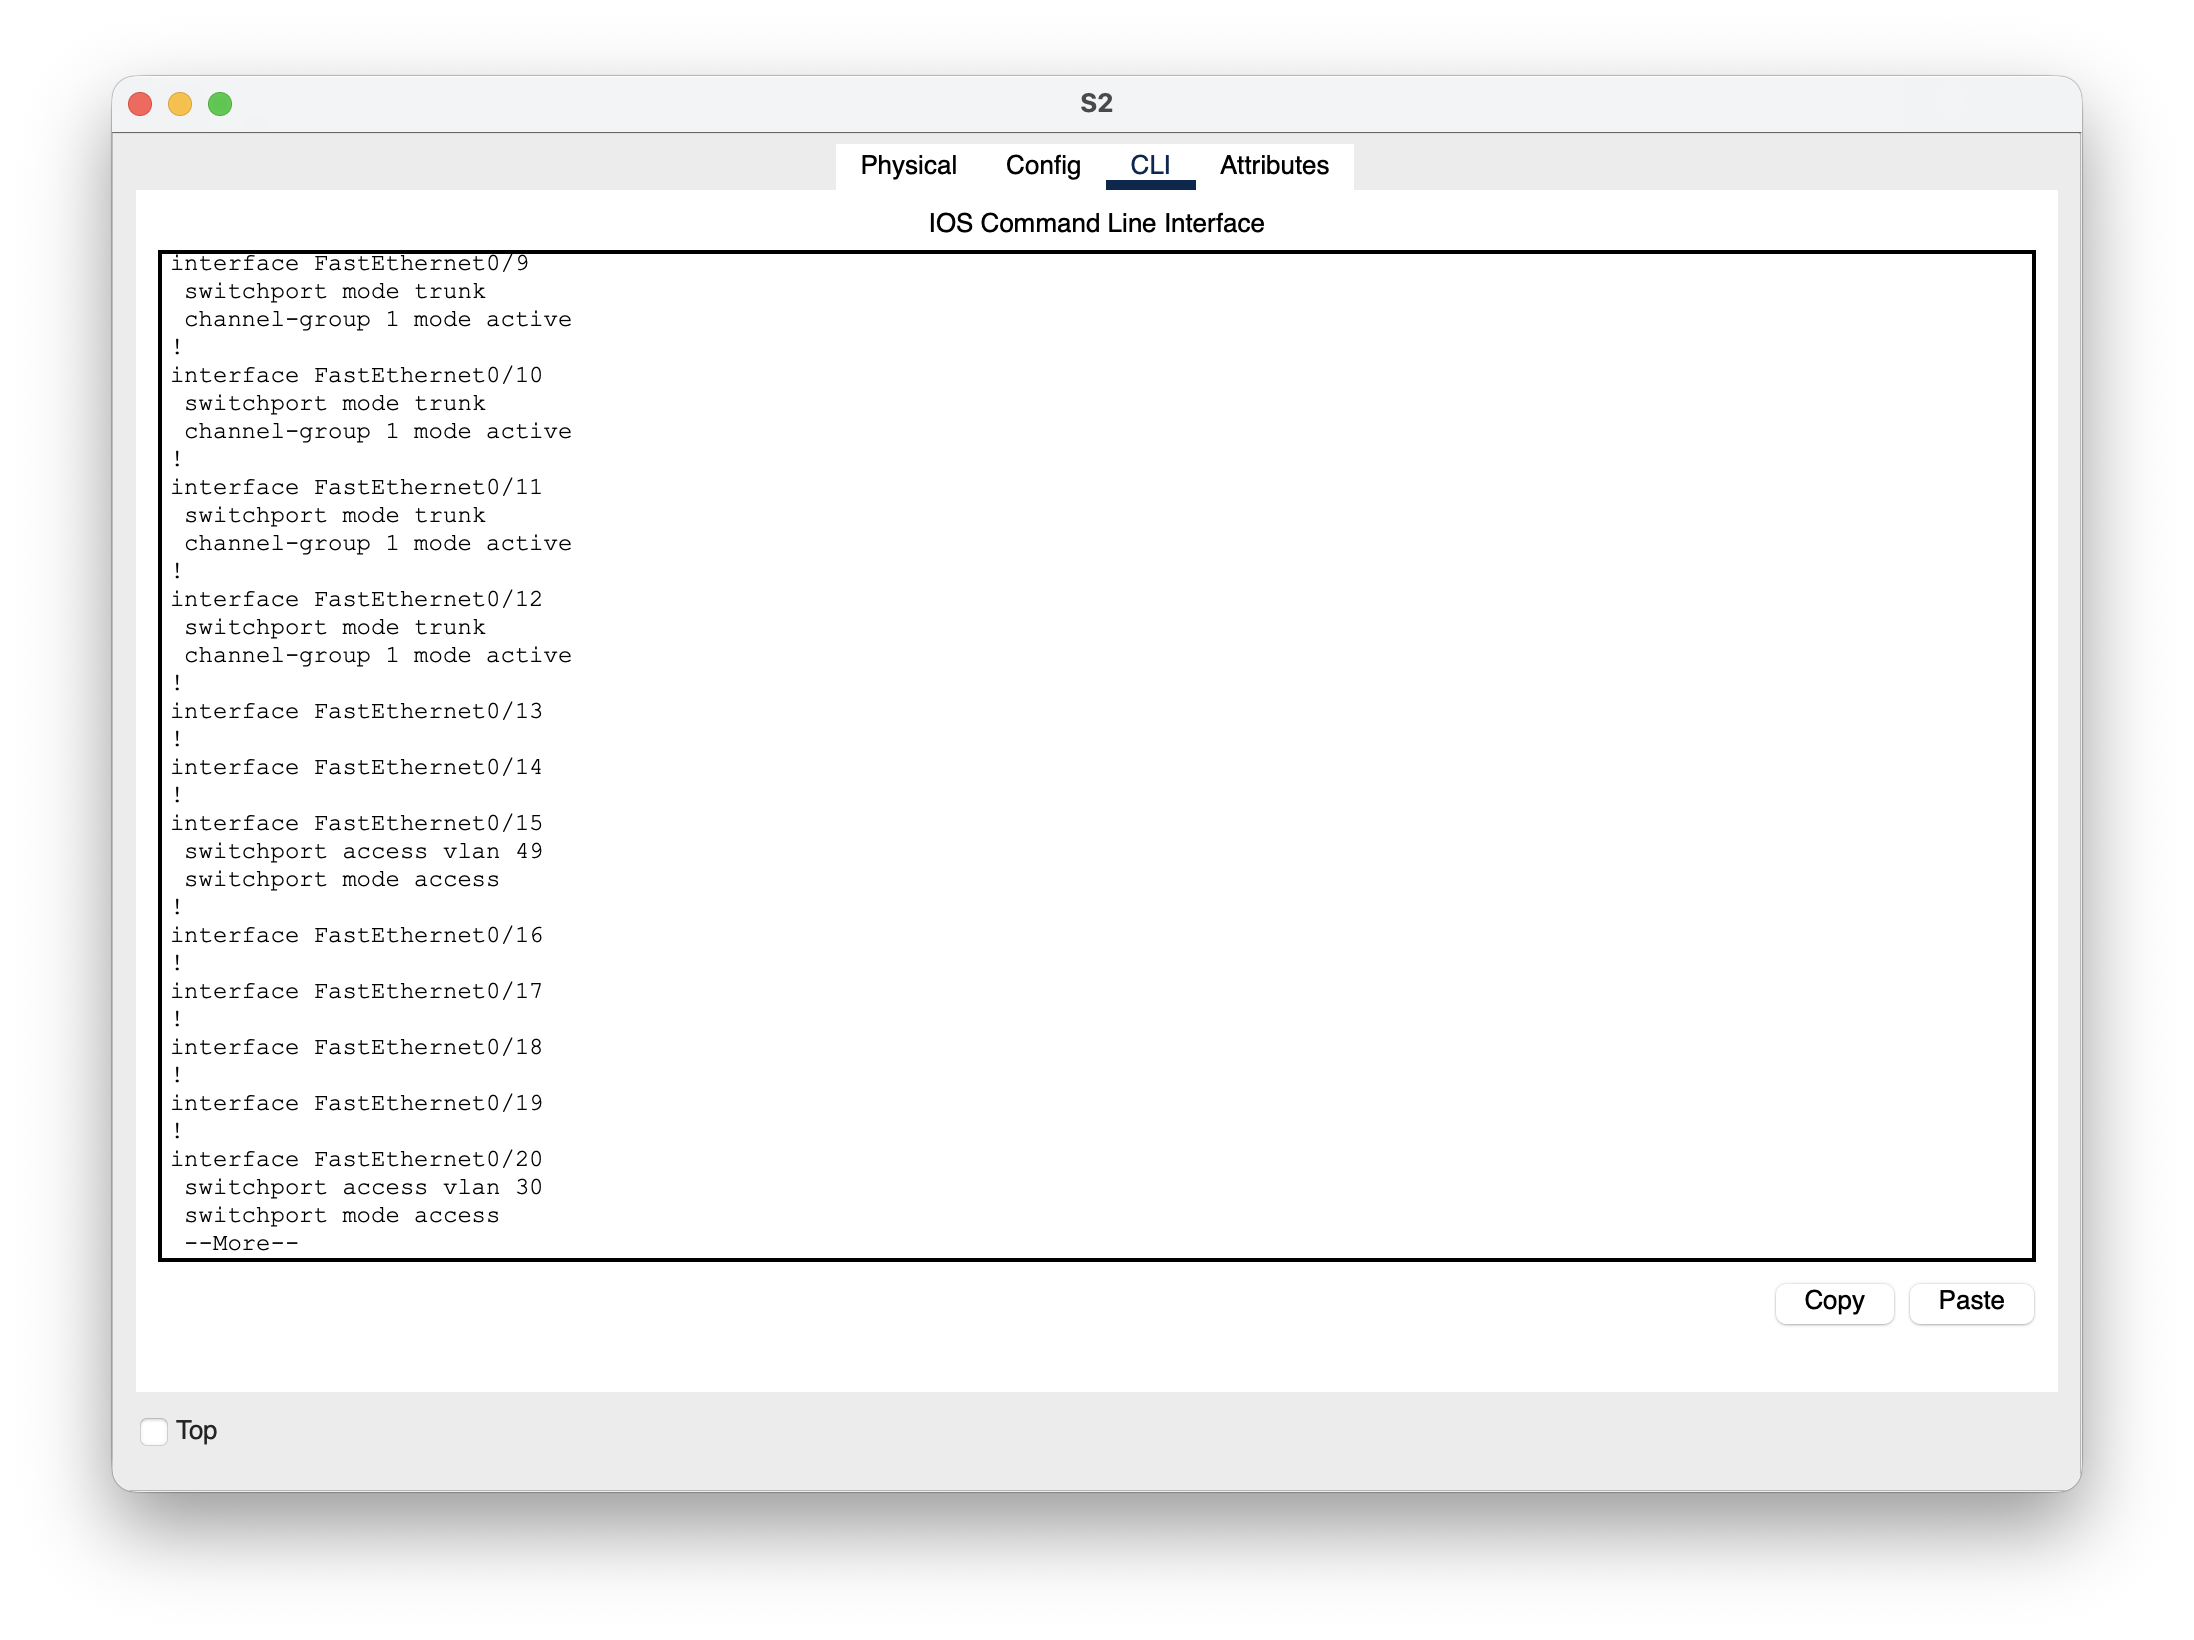
\includegraphics[width=0.8\textwidth]{running-configS2(2).png}
  \caption{Configuración activa S2 (continuación)}\label{fig:running-configS2(2)}
\end{figure}

\section{VLAN, DHCP y ETHERCHANNEL}

\subsection{VLAN}
Ejecutamos el comando \textit{show vlan brief} en S1 y S2 para que nos muestren la configuración 
actual de VLANS

\begin{figure}[H]
  \centering
  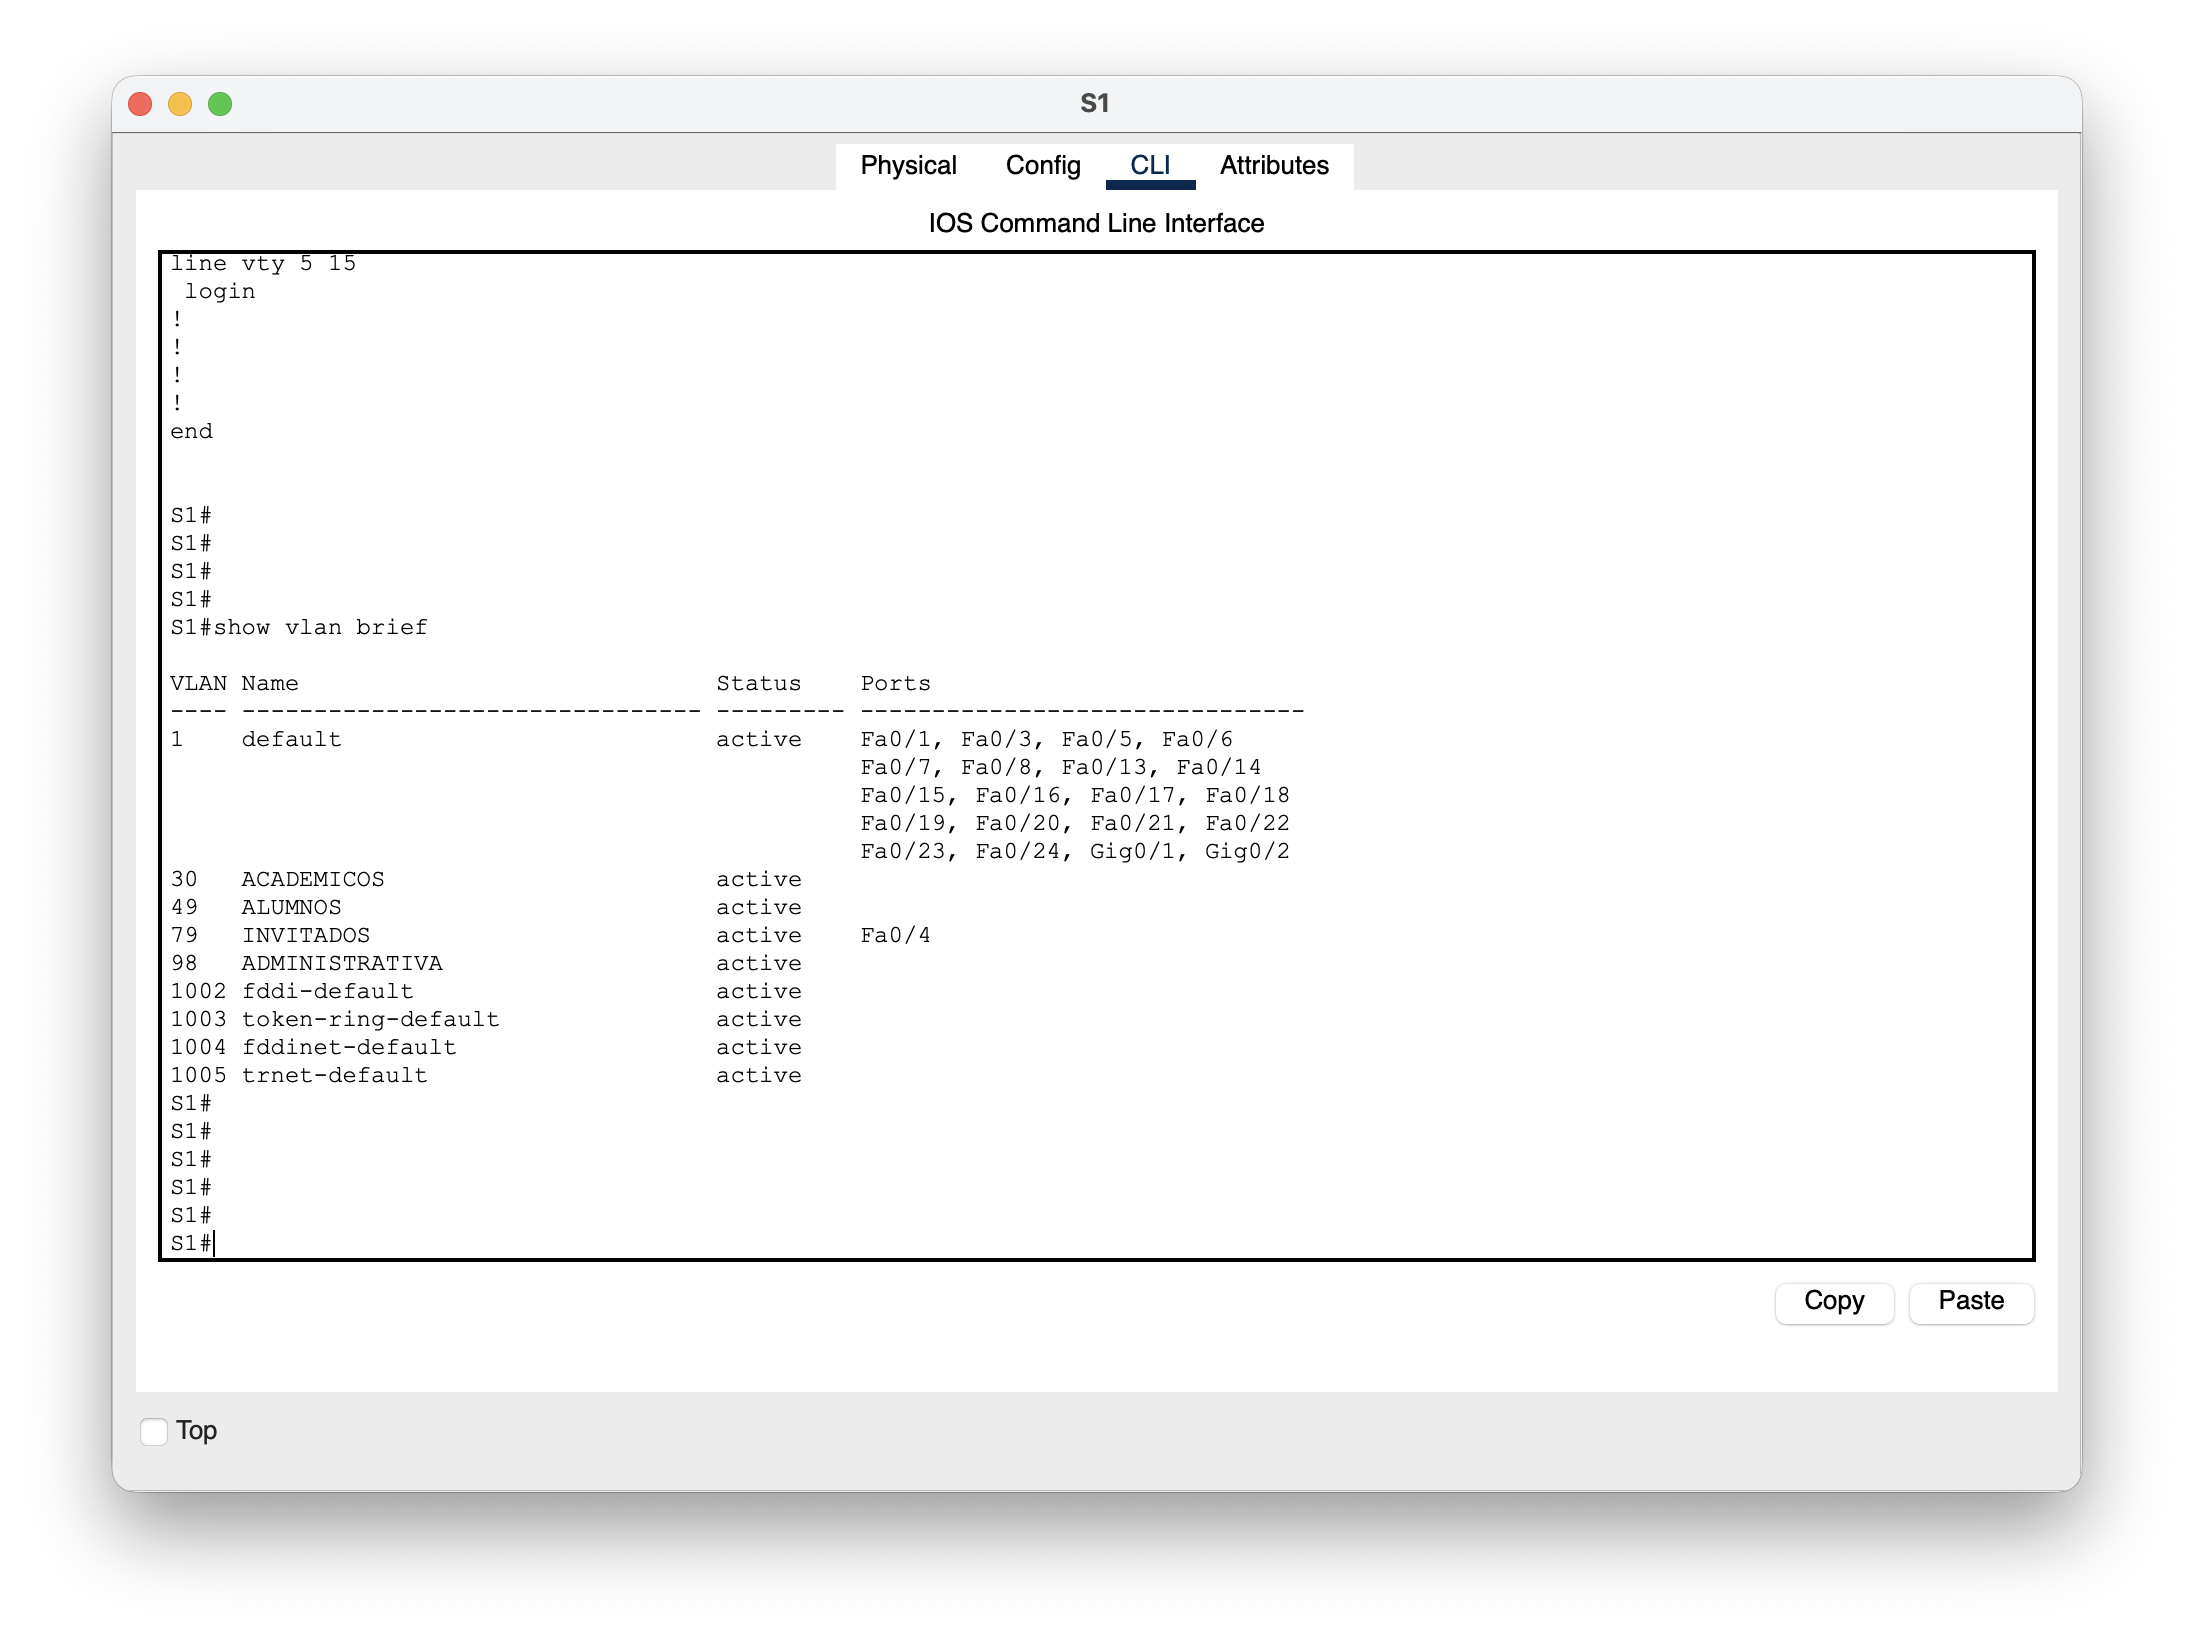
\includegraphics[width=0.8\textwidth]{vlanS1.png}
  \caption{Configuración de vlan en S1}\label{fig:vlanS1}
\end{figure}

\begin{figure}[H]
  \centering
  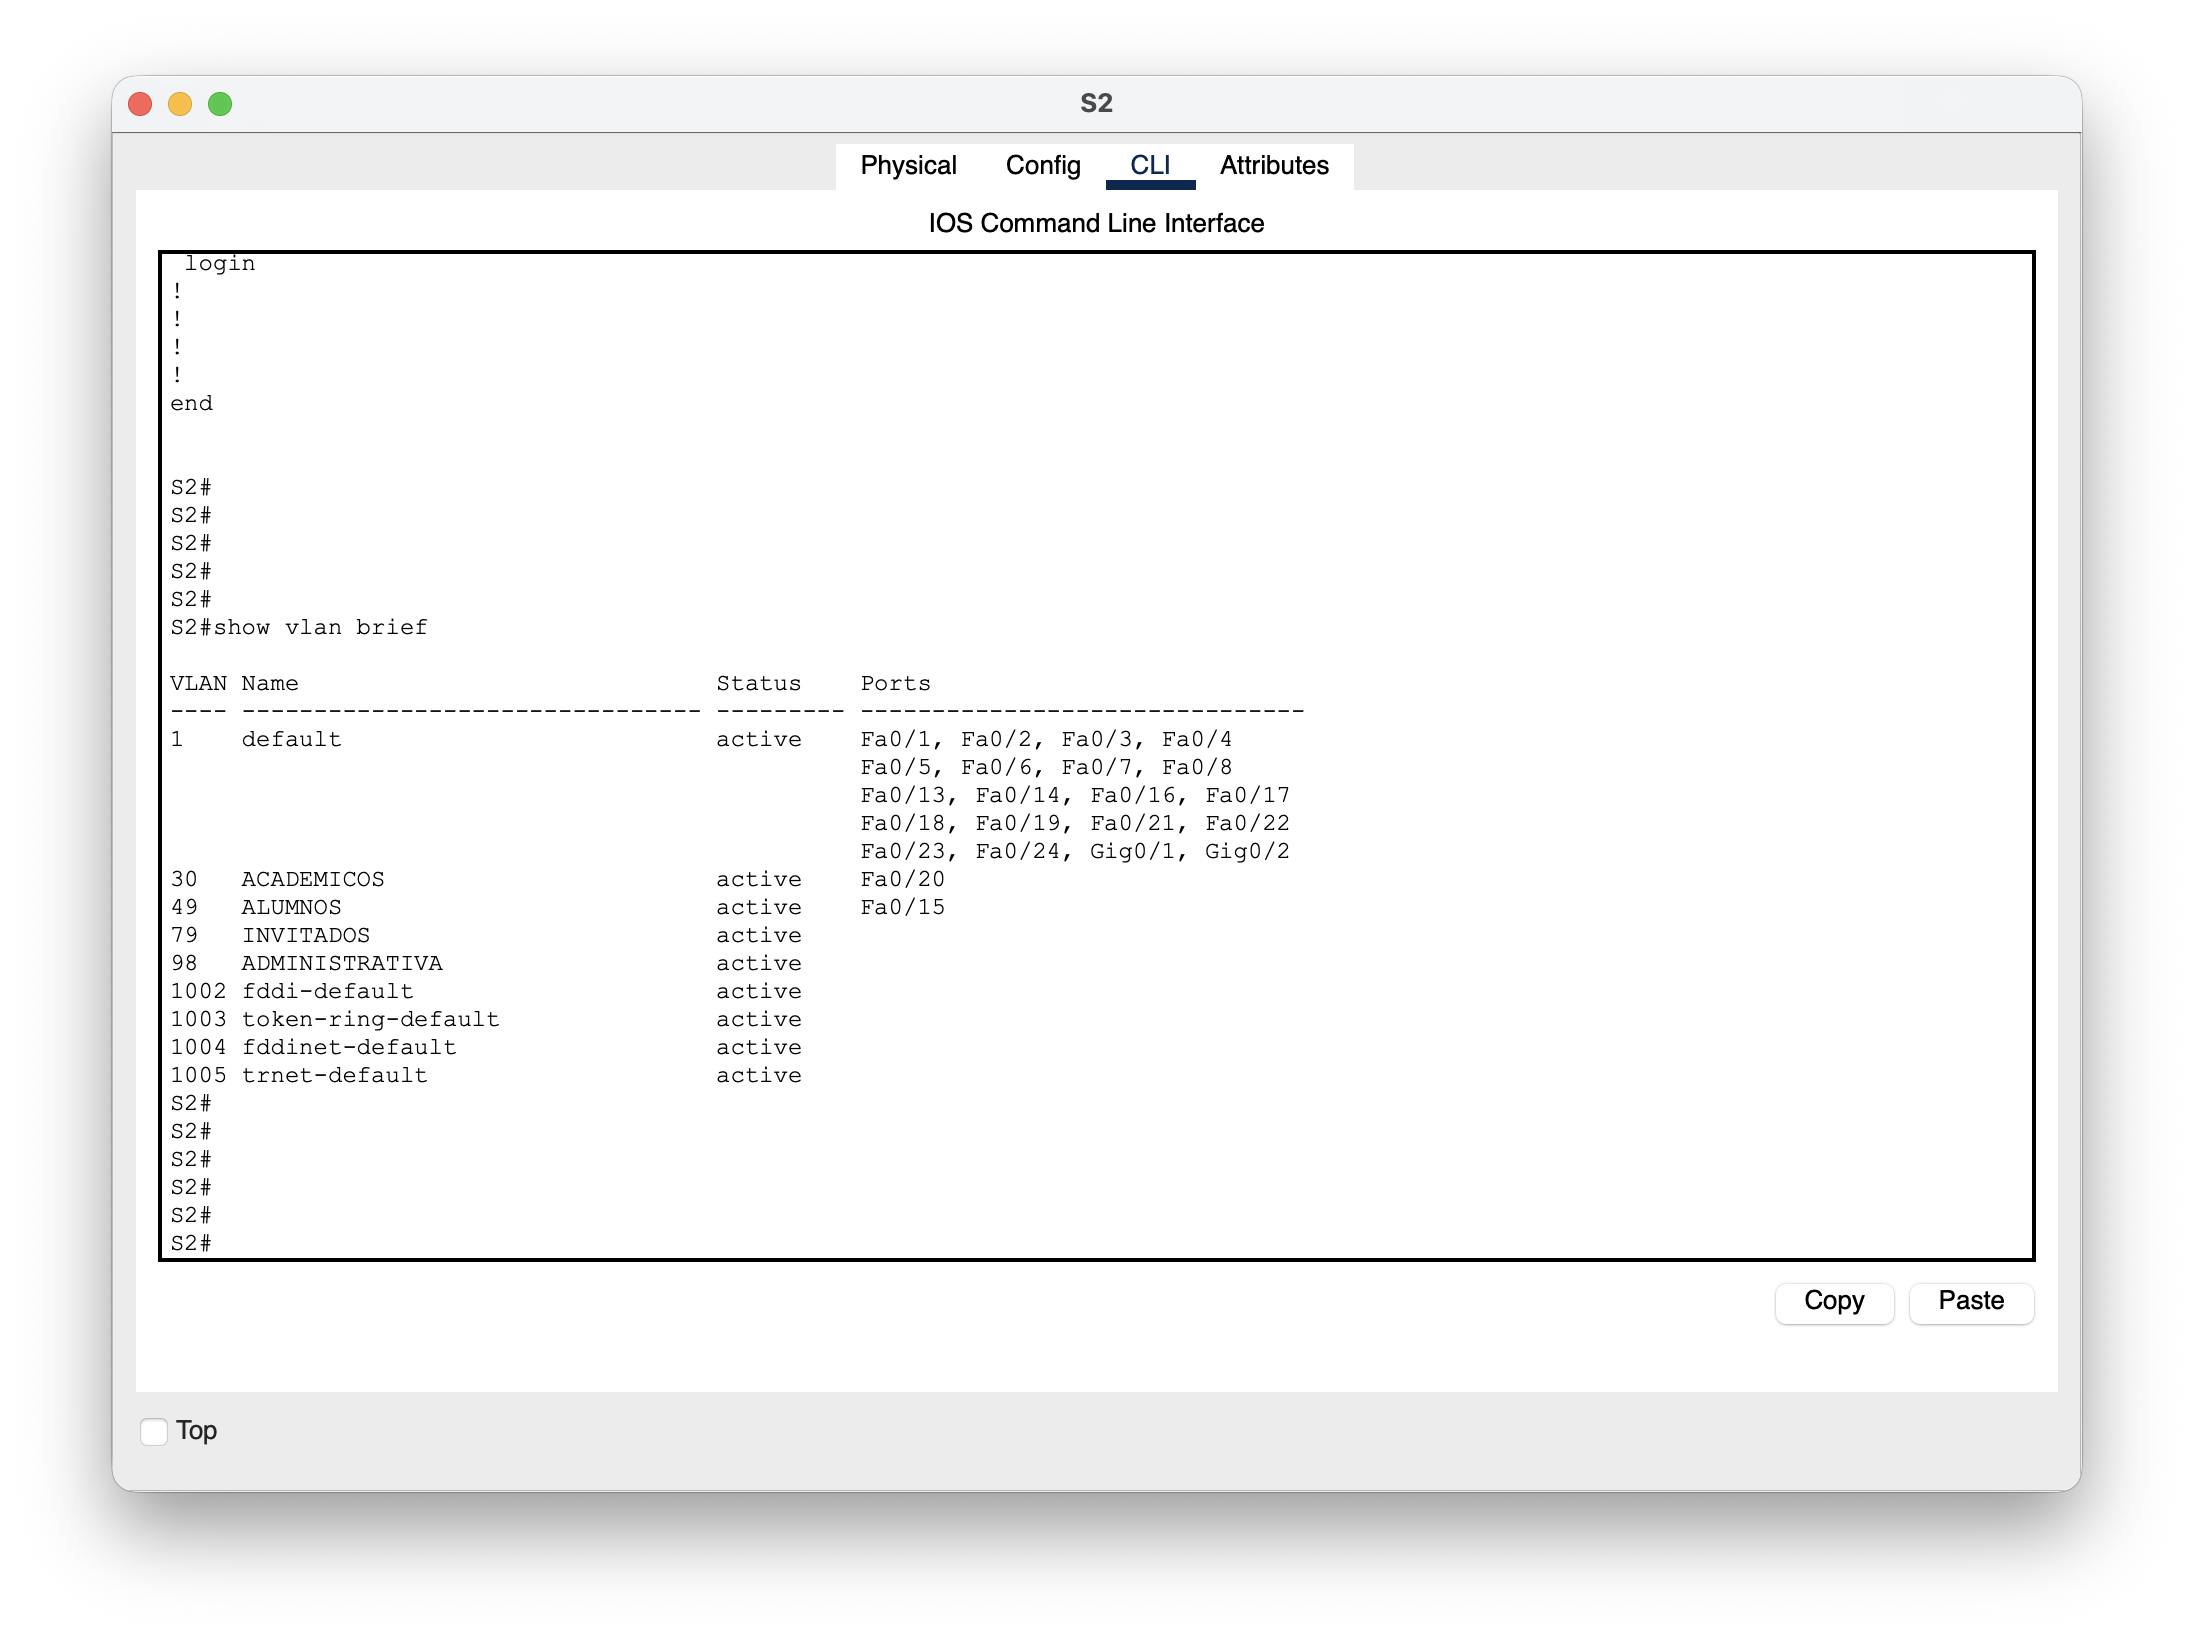
\includegraphics[width=0.8\textwidth]{vlanS2.png}
  \caption{Configuración de vlan en S2}\label{fig:vlanS2}
\end{figure}

\subsection{DHCP}
Ejecutamos el comando \textit{show ip dhcp pool} en R1 para que nos muestre la configuración 
actual del DHCP

\begin{figure}[H]
  \centering
  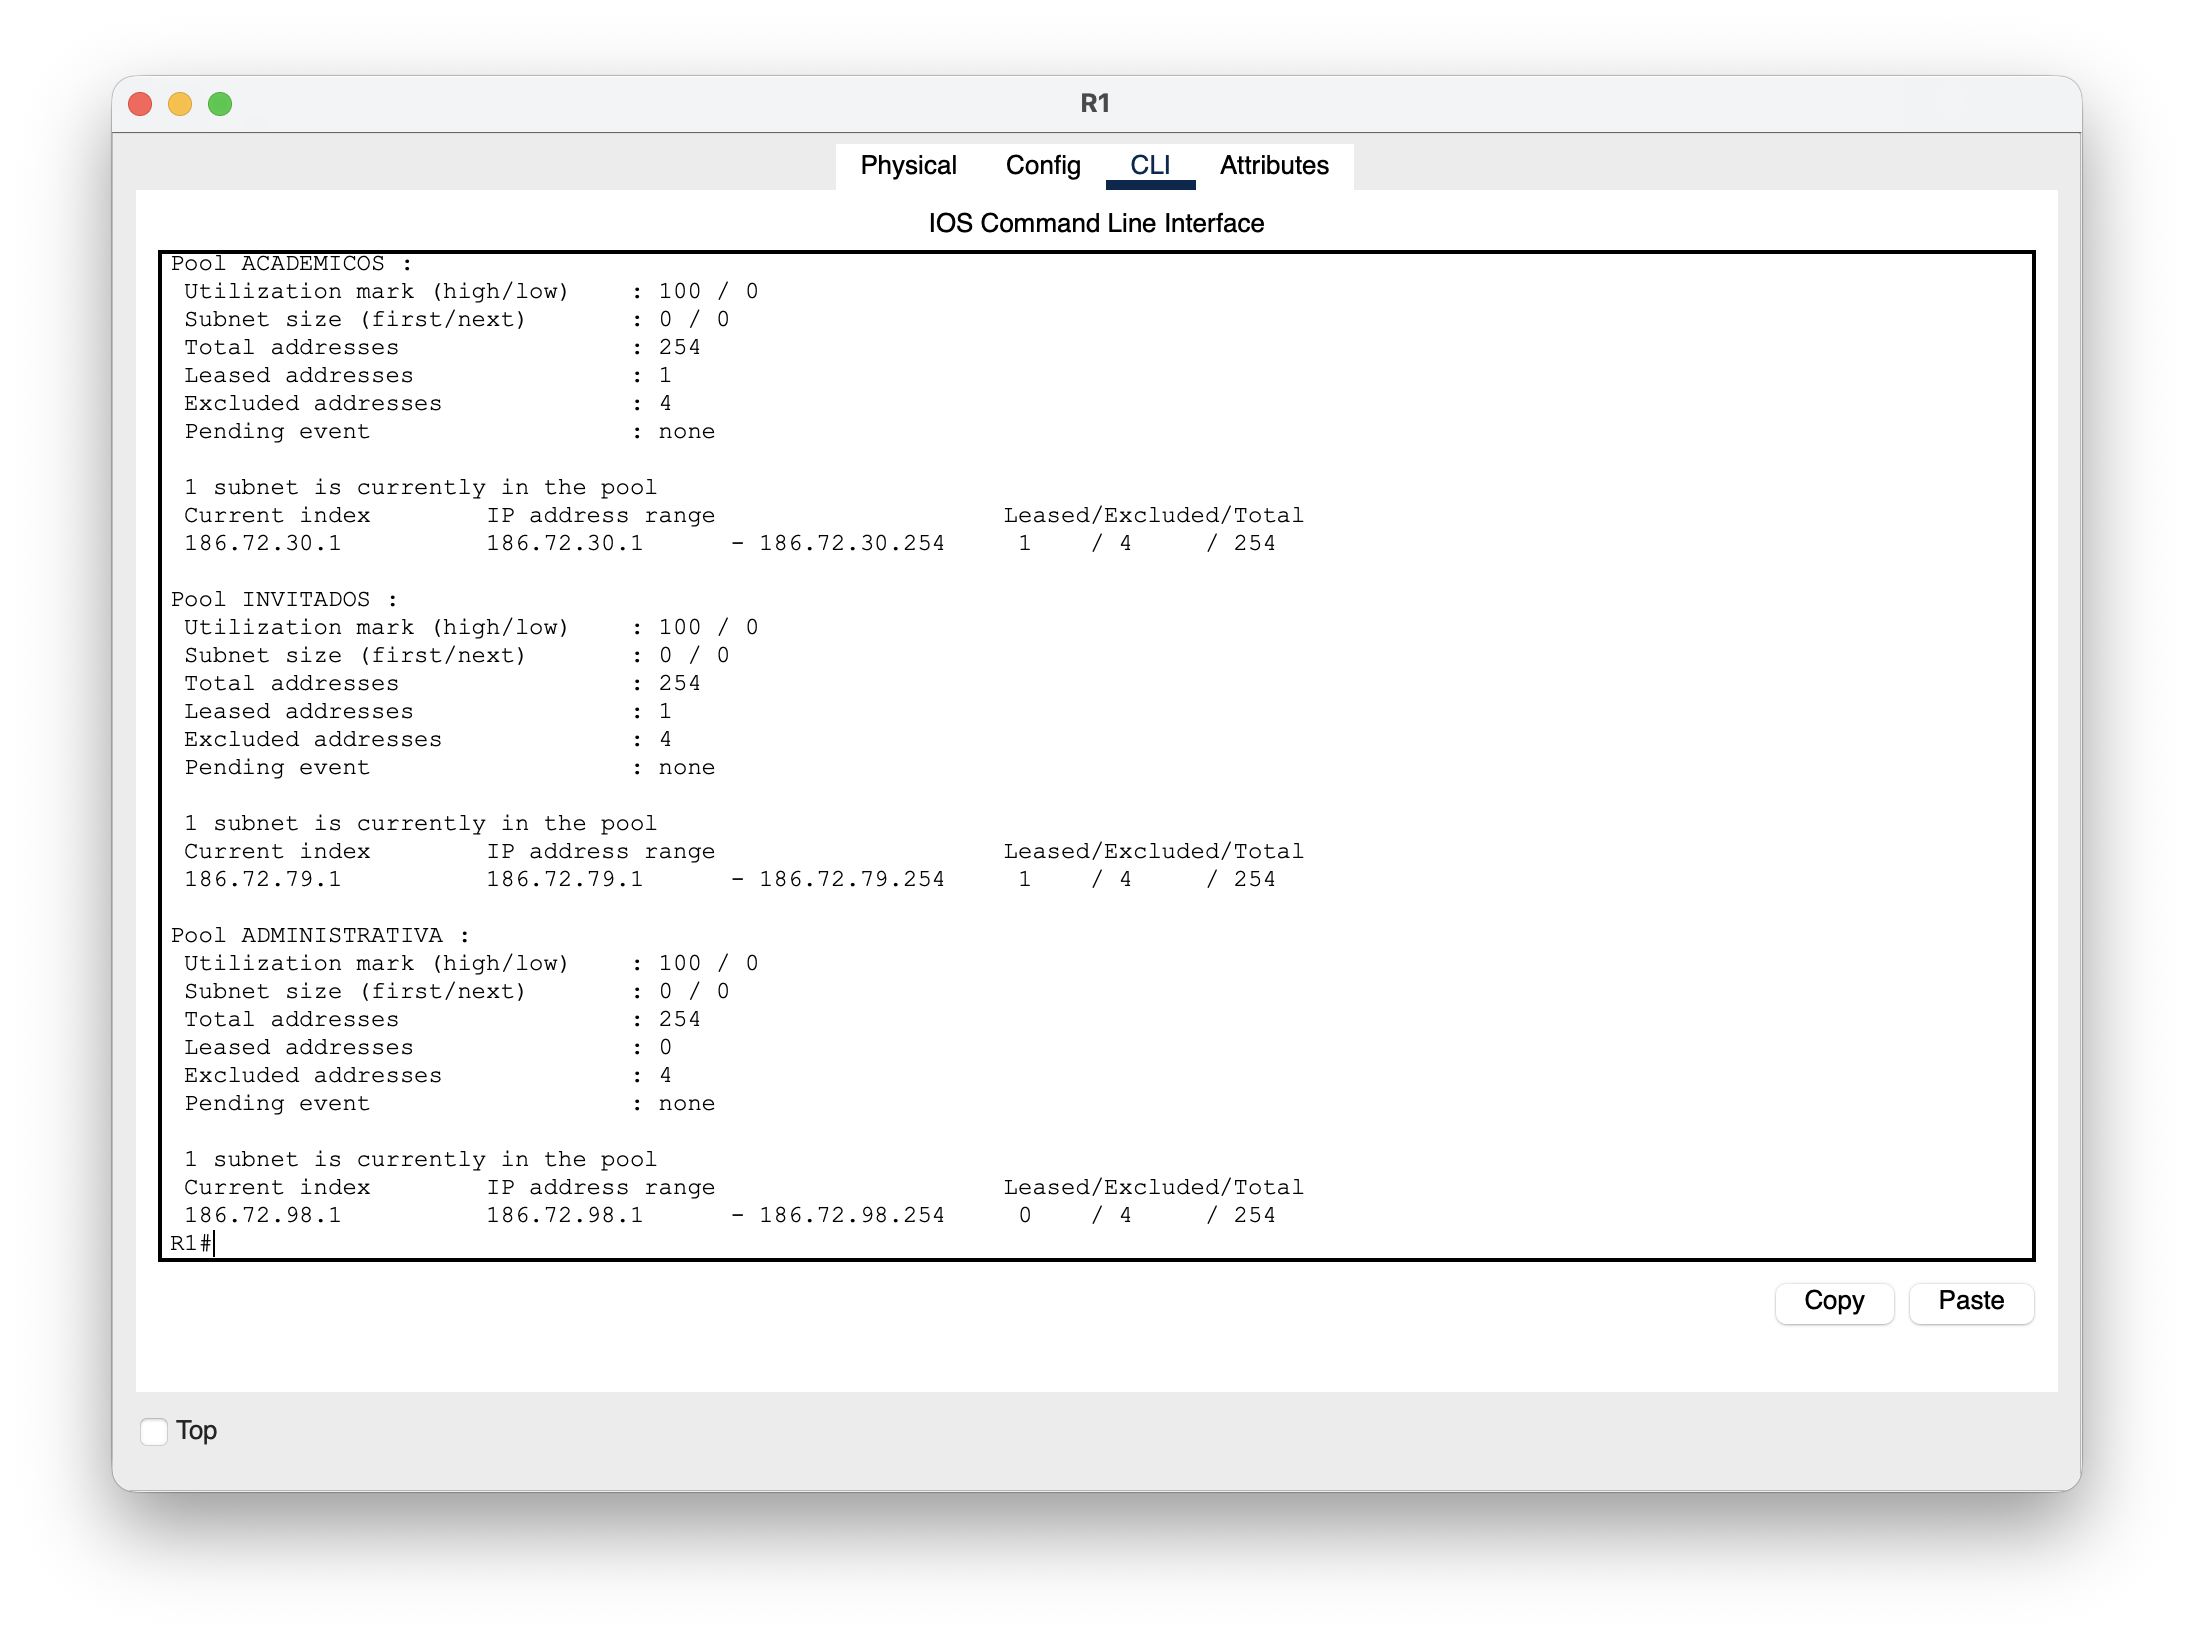
\includegraphics[width=0.8\textwidth]{dhcpR1.png}
  \caption{Configuración del DHCP en R1}\label{fig:dhcpR1}
\end{figure}

\subsection{ETHERCHANNEL}
Ejecutamos el comando \textit{show etherchannel summary} en cada Switch para que nos muestren la configuración 
actual del EtherChannel

\begin{figure}[H]
  \centering
  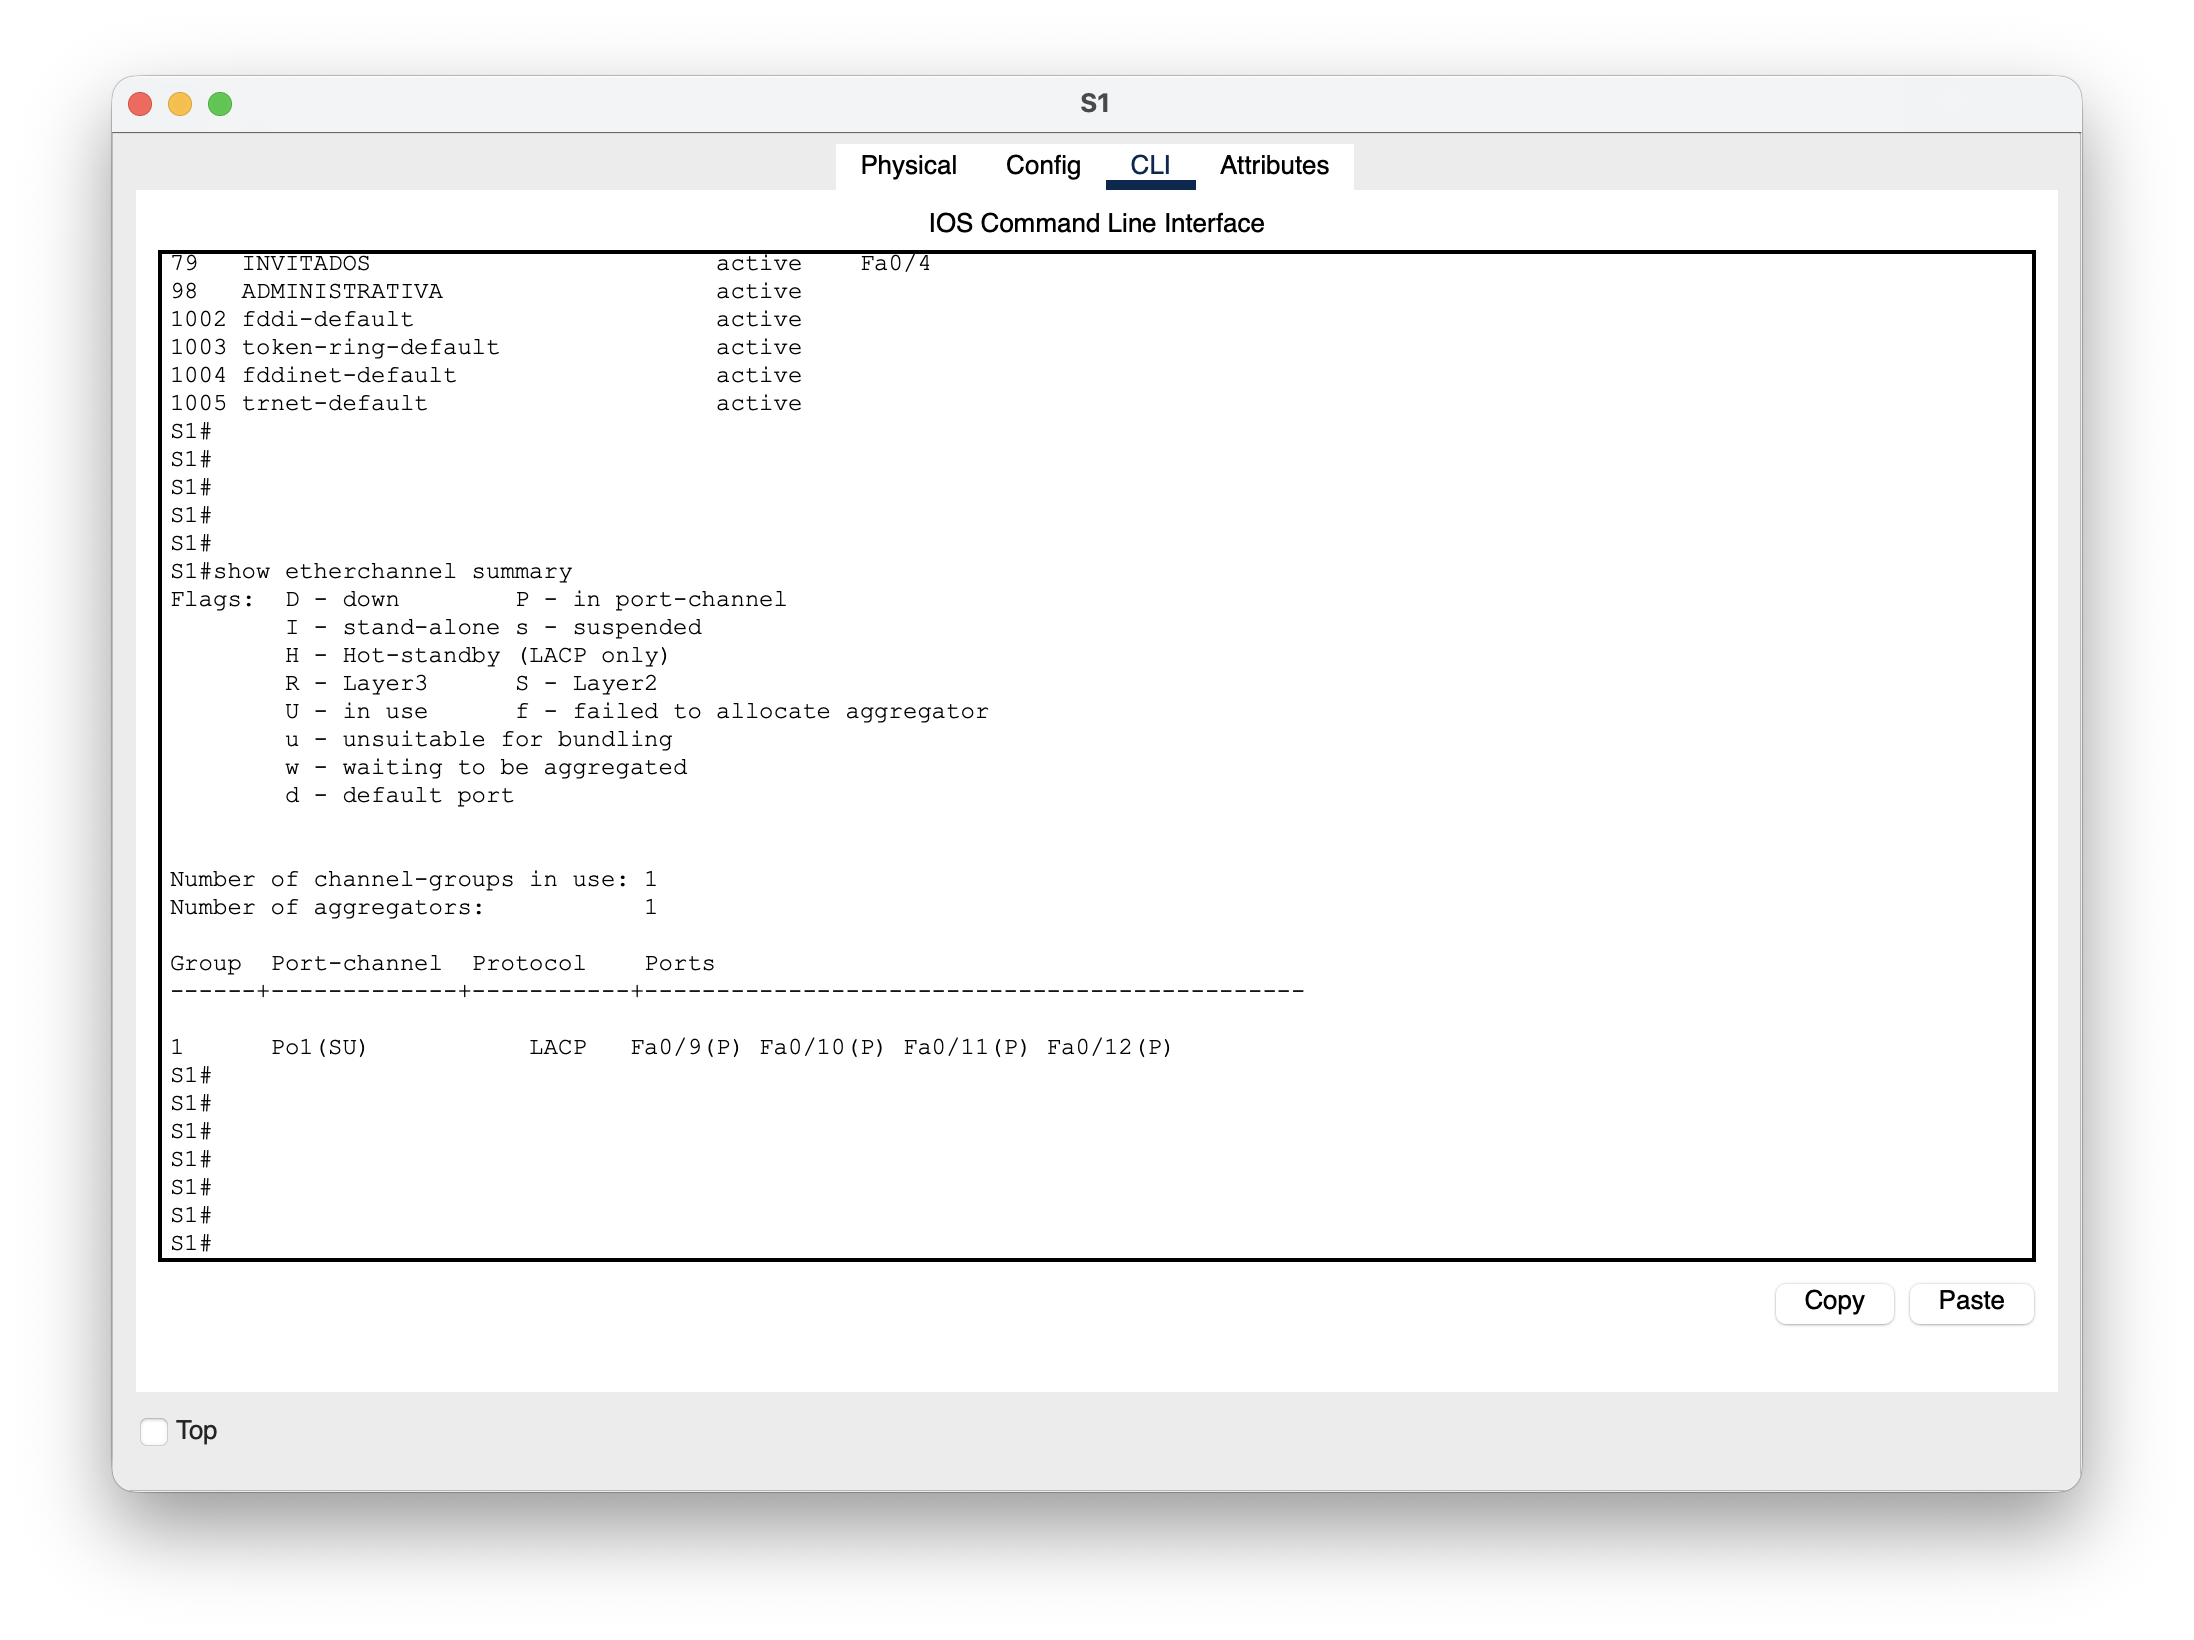
\includegraphics[width=0.8\textwidth]{etherchannelS1.png}
  \caption{Configuración del etherchannel en S1}\label{fig:etherchannelS1}
\end{figure}

\begin{figure}[H]
  \centering
  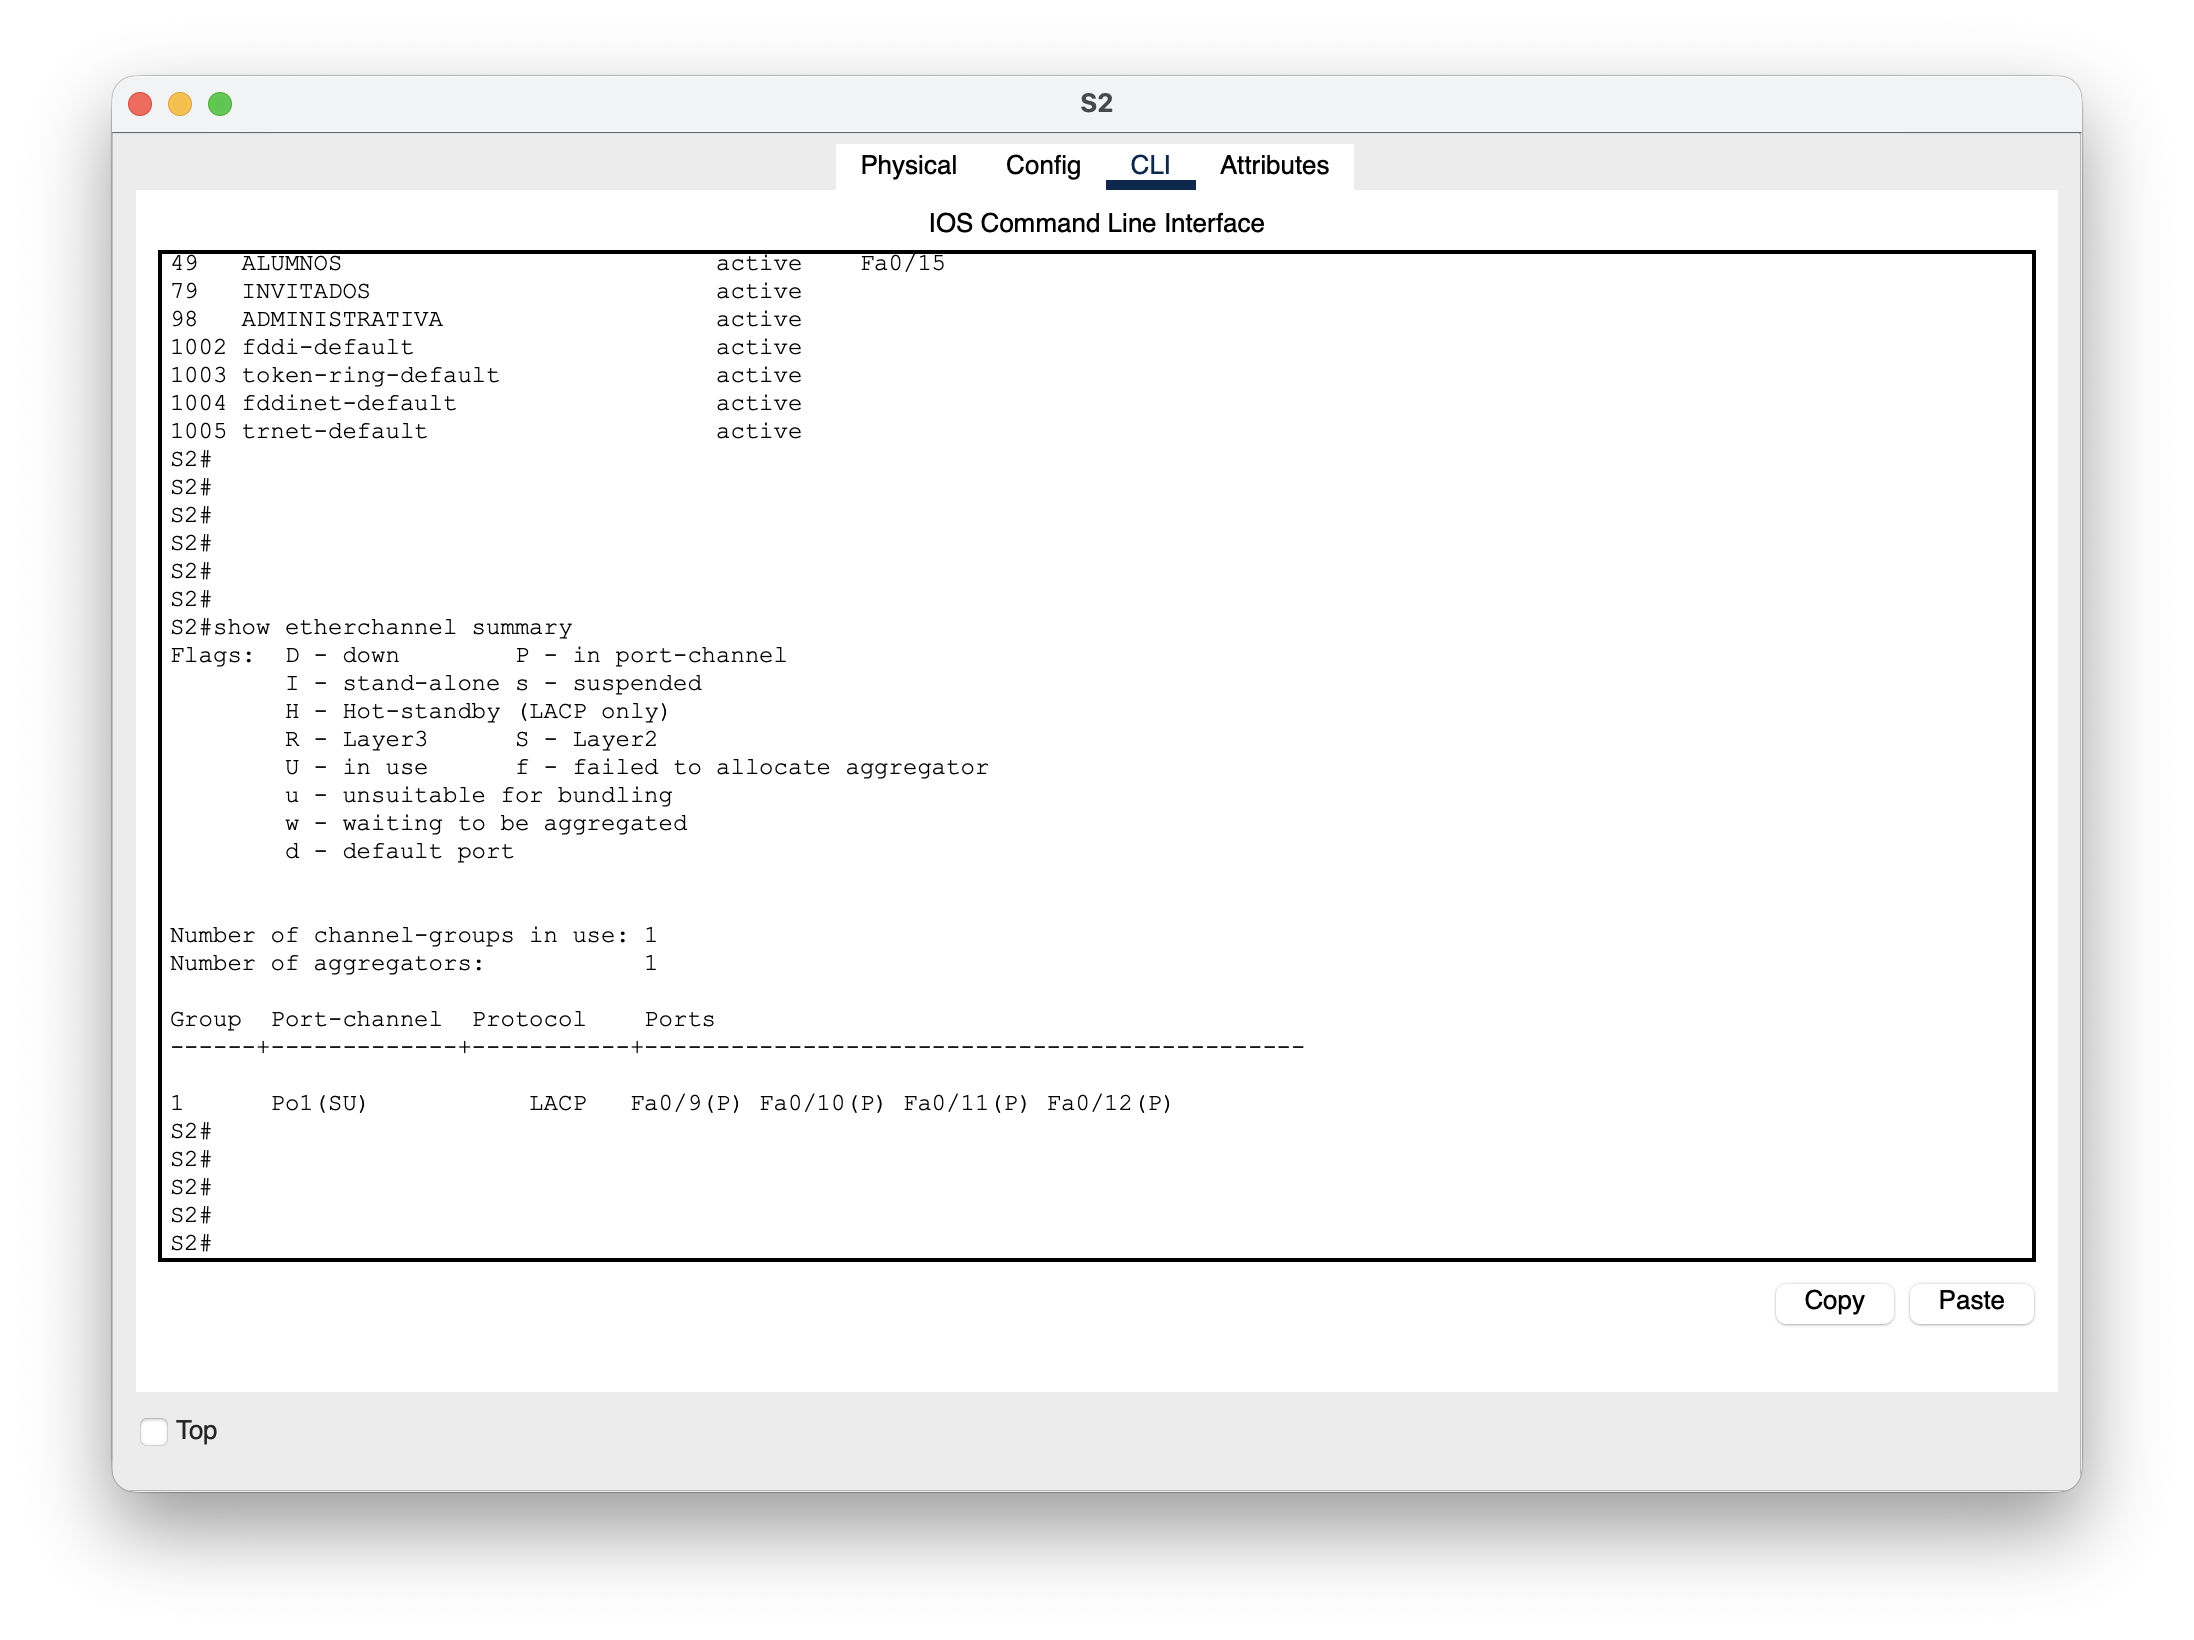
\includegraphics[width=0.8\textwidth]{etherchannelS2.png}
  \caption{Configuración del etherchannel en S2}\label{fig:etherchannelS2}
\end{figure}

\section{Práctica con equipo físico}
A continuación se muestran imágenes de la realización, configuración y resultados de la práctica 
realizada en equipo físico bajo la supervición y revisión de los becarios del laboratorio de redes.

\begin{figure}[H]
  \centering
  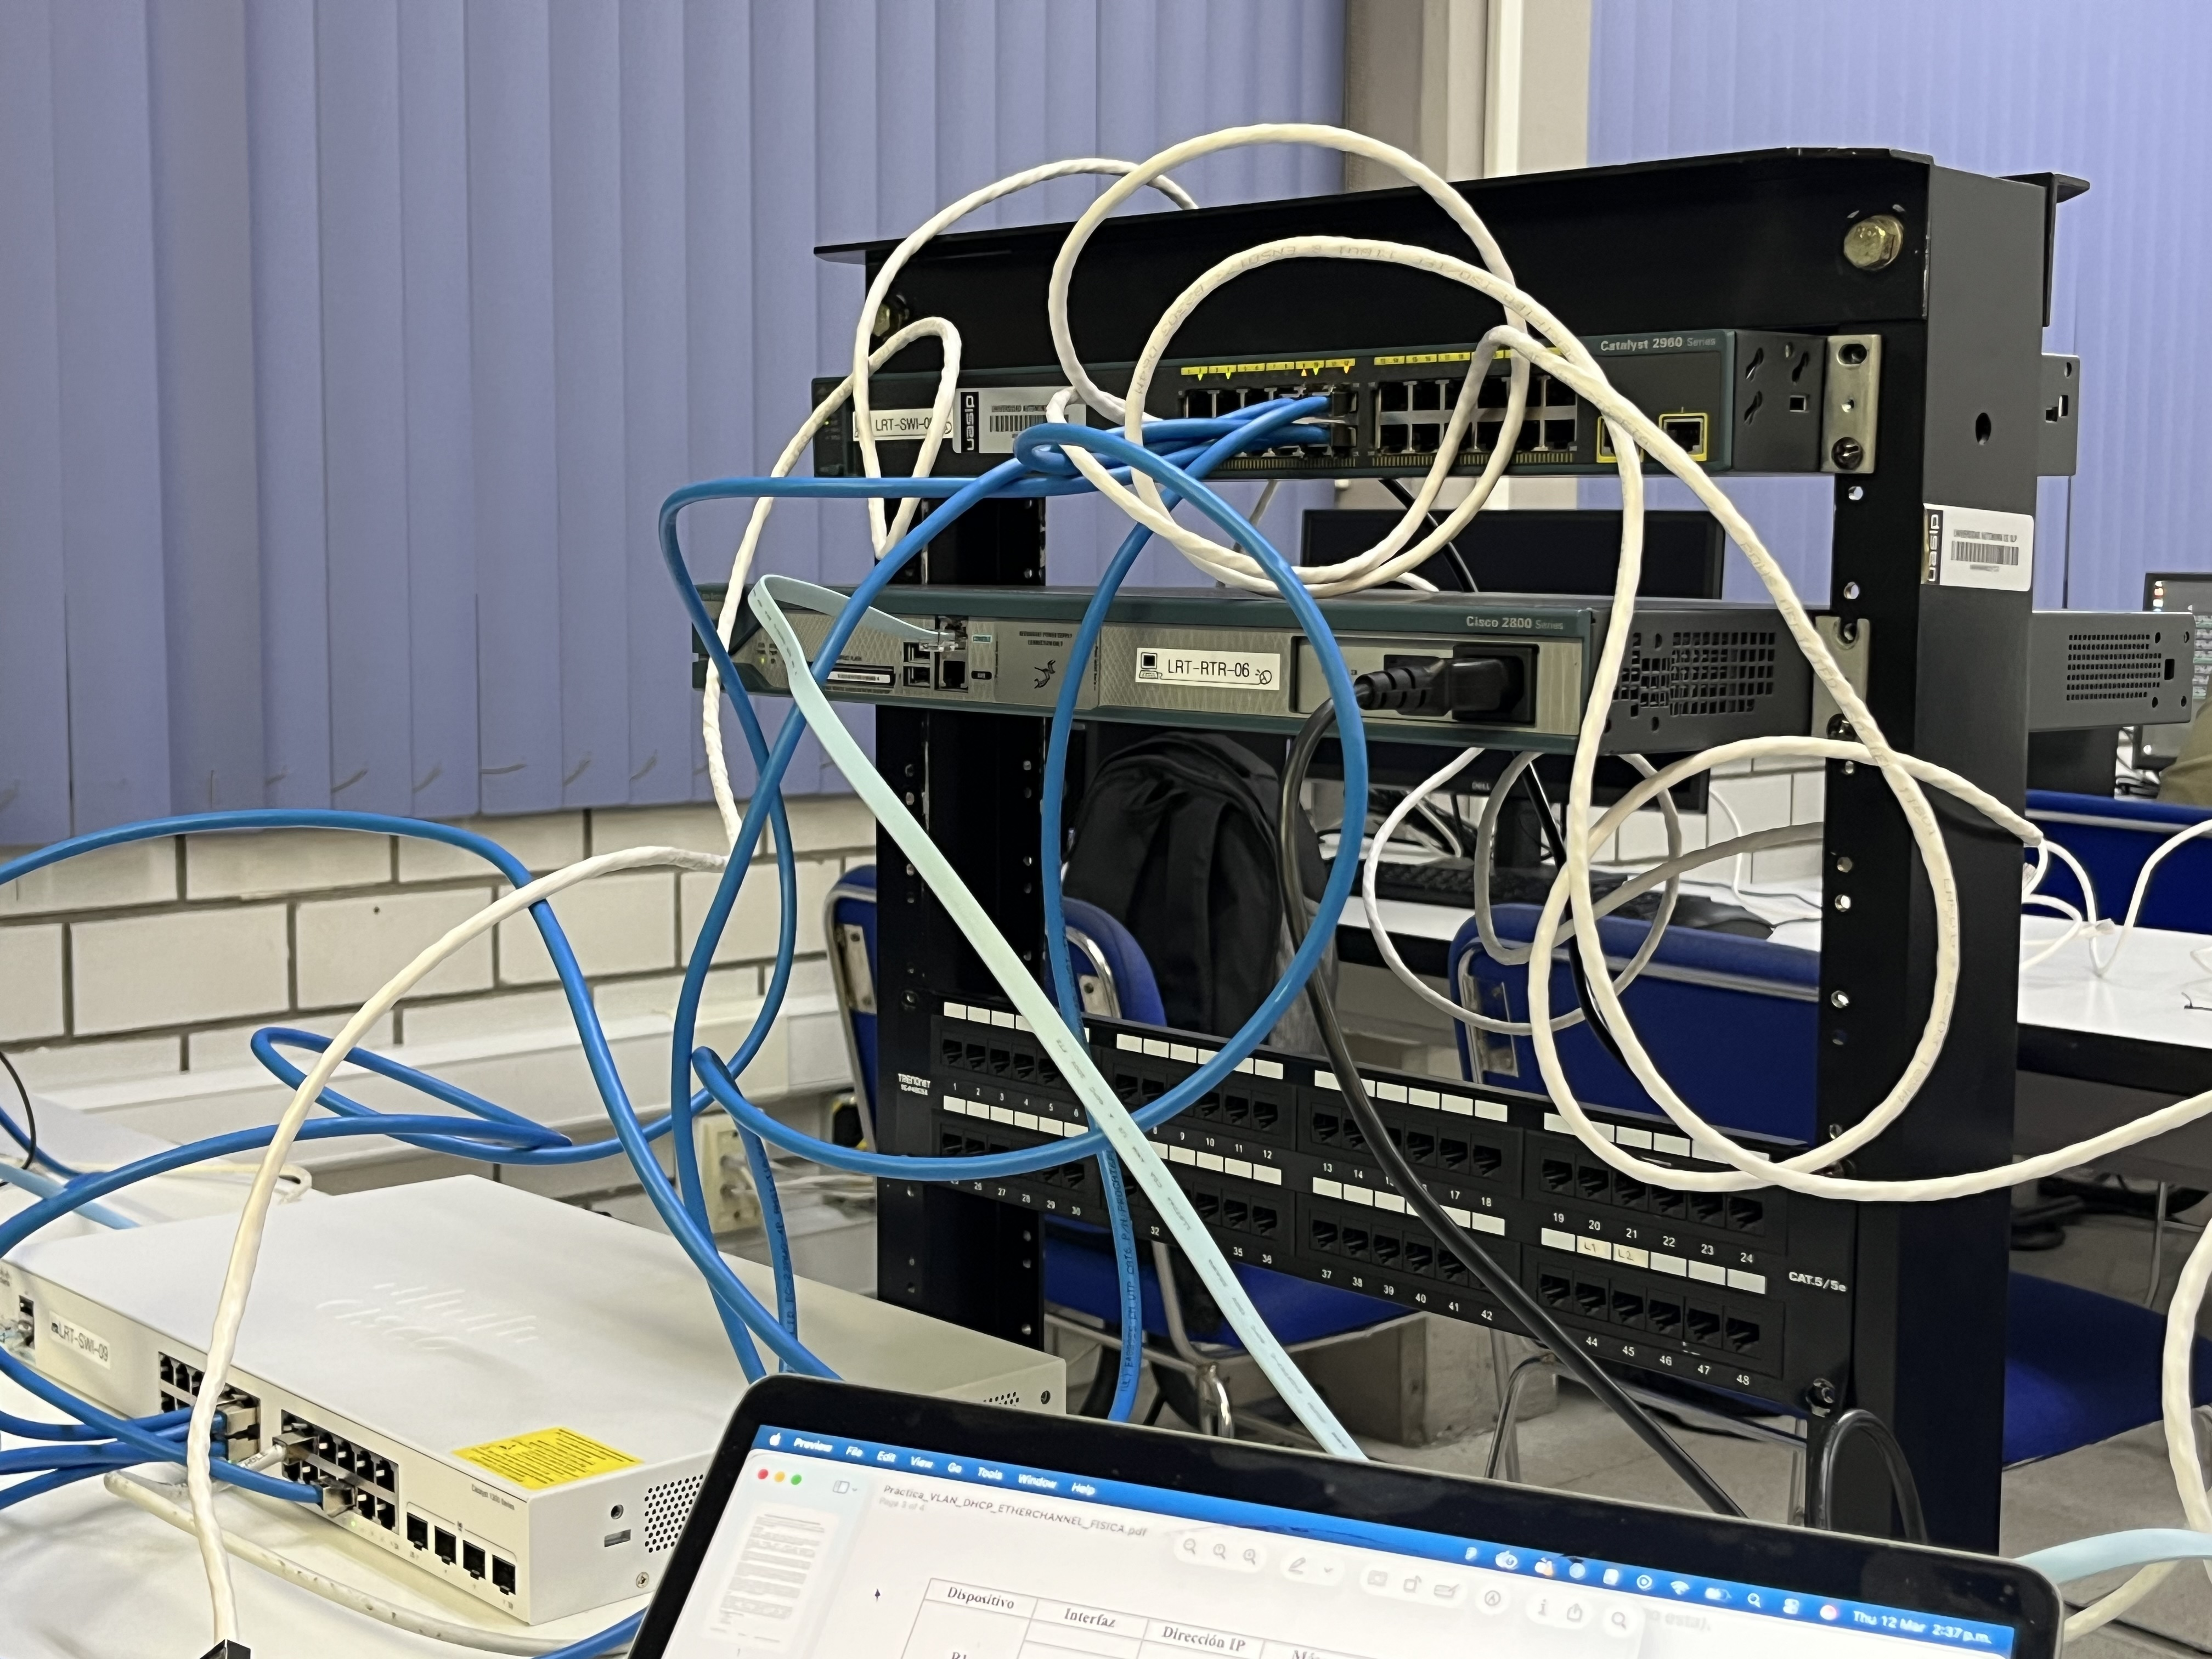
\includegraphics[width=0.8\textwidth]{practfis1.jpg}
  \caption{Evidencia de realización de práctica en equipo físico}\label{fig:practfis1}
\end{figure}

\begin{figure}[H]
  \centering
  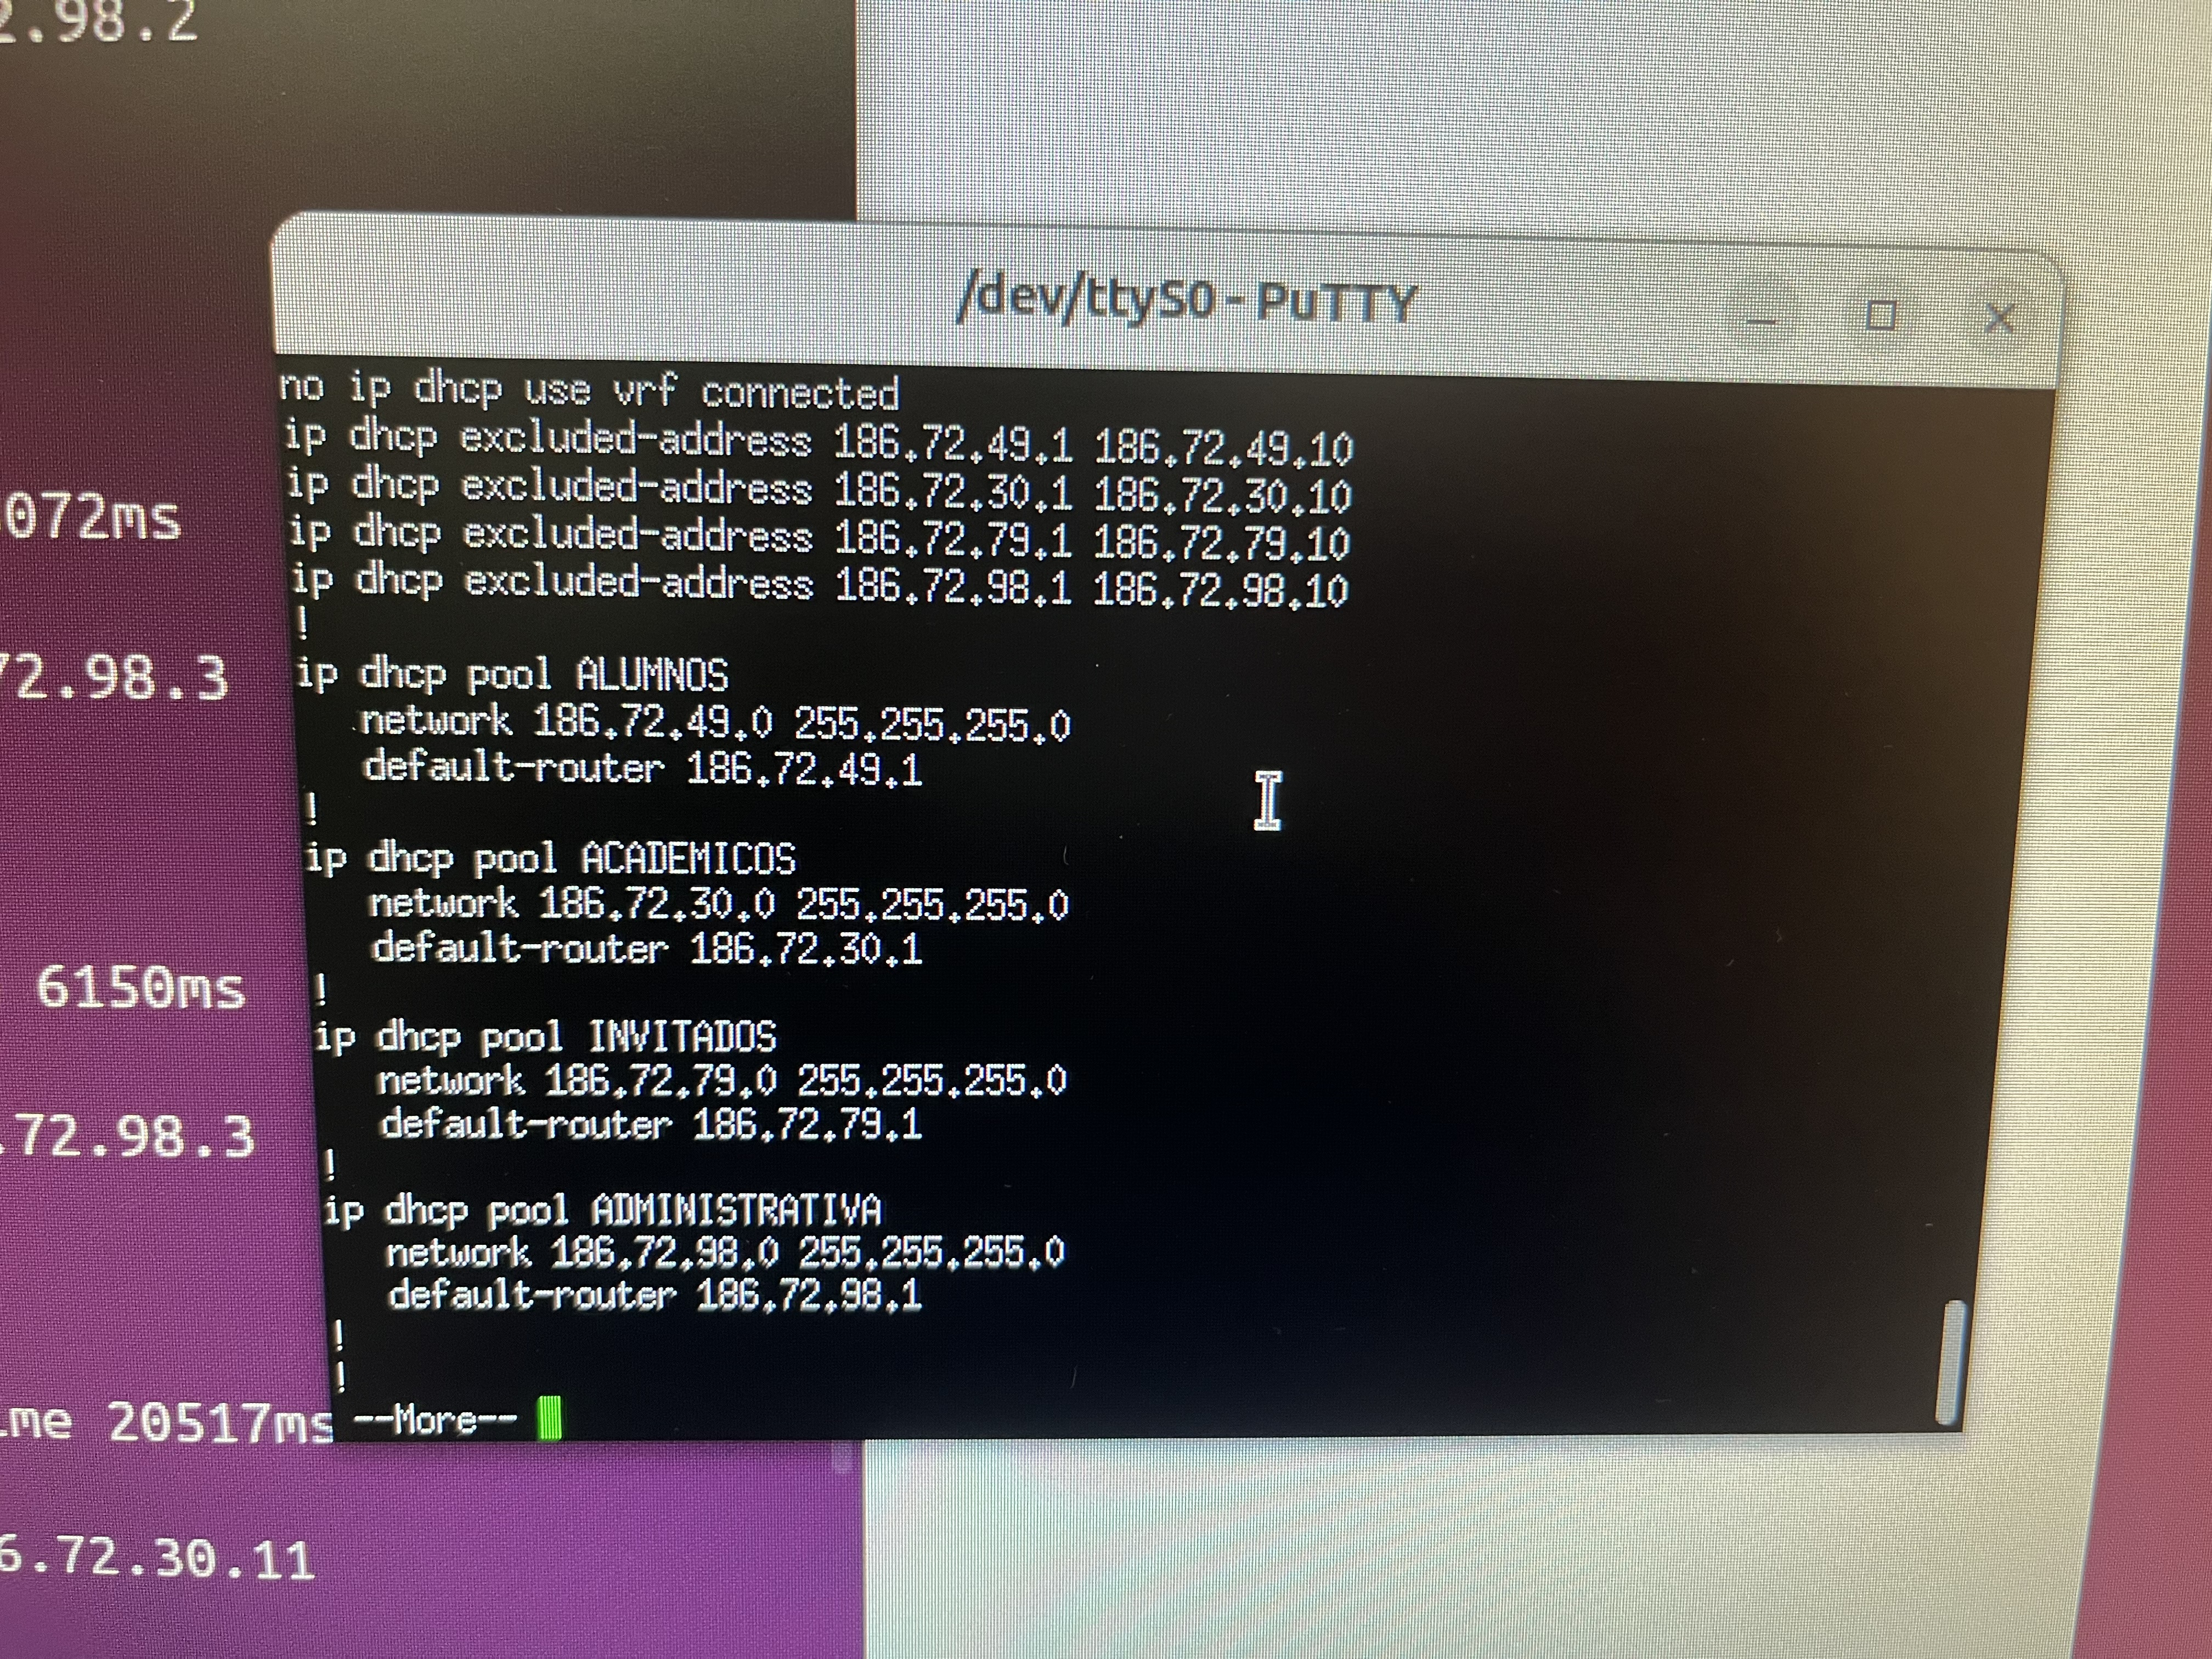
\includegraphics[width=0.8\textwidth]{practfis2.jpg}
  \caption{Evidencia de realización de práctica en equipo físico}\label{fig:practfis2}
\end{figure}

\begin{figure}[H]
  \centering
  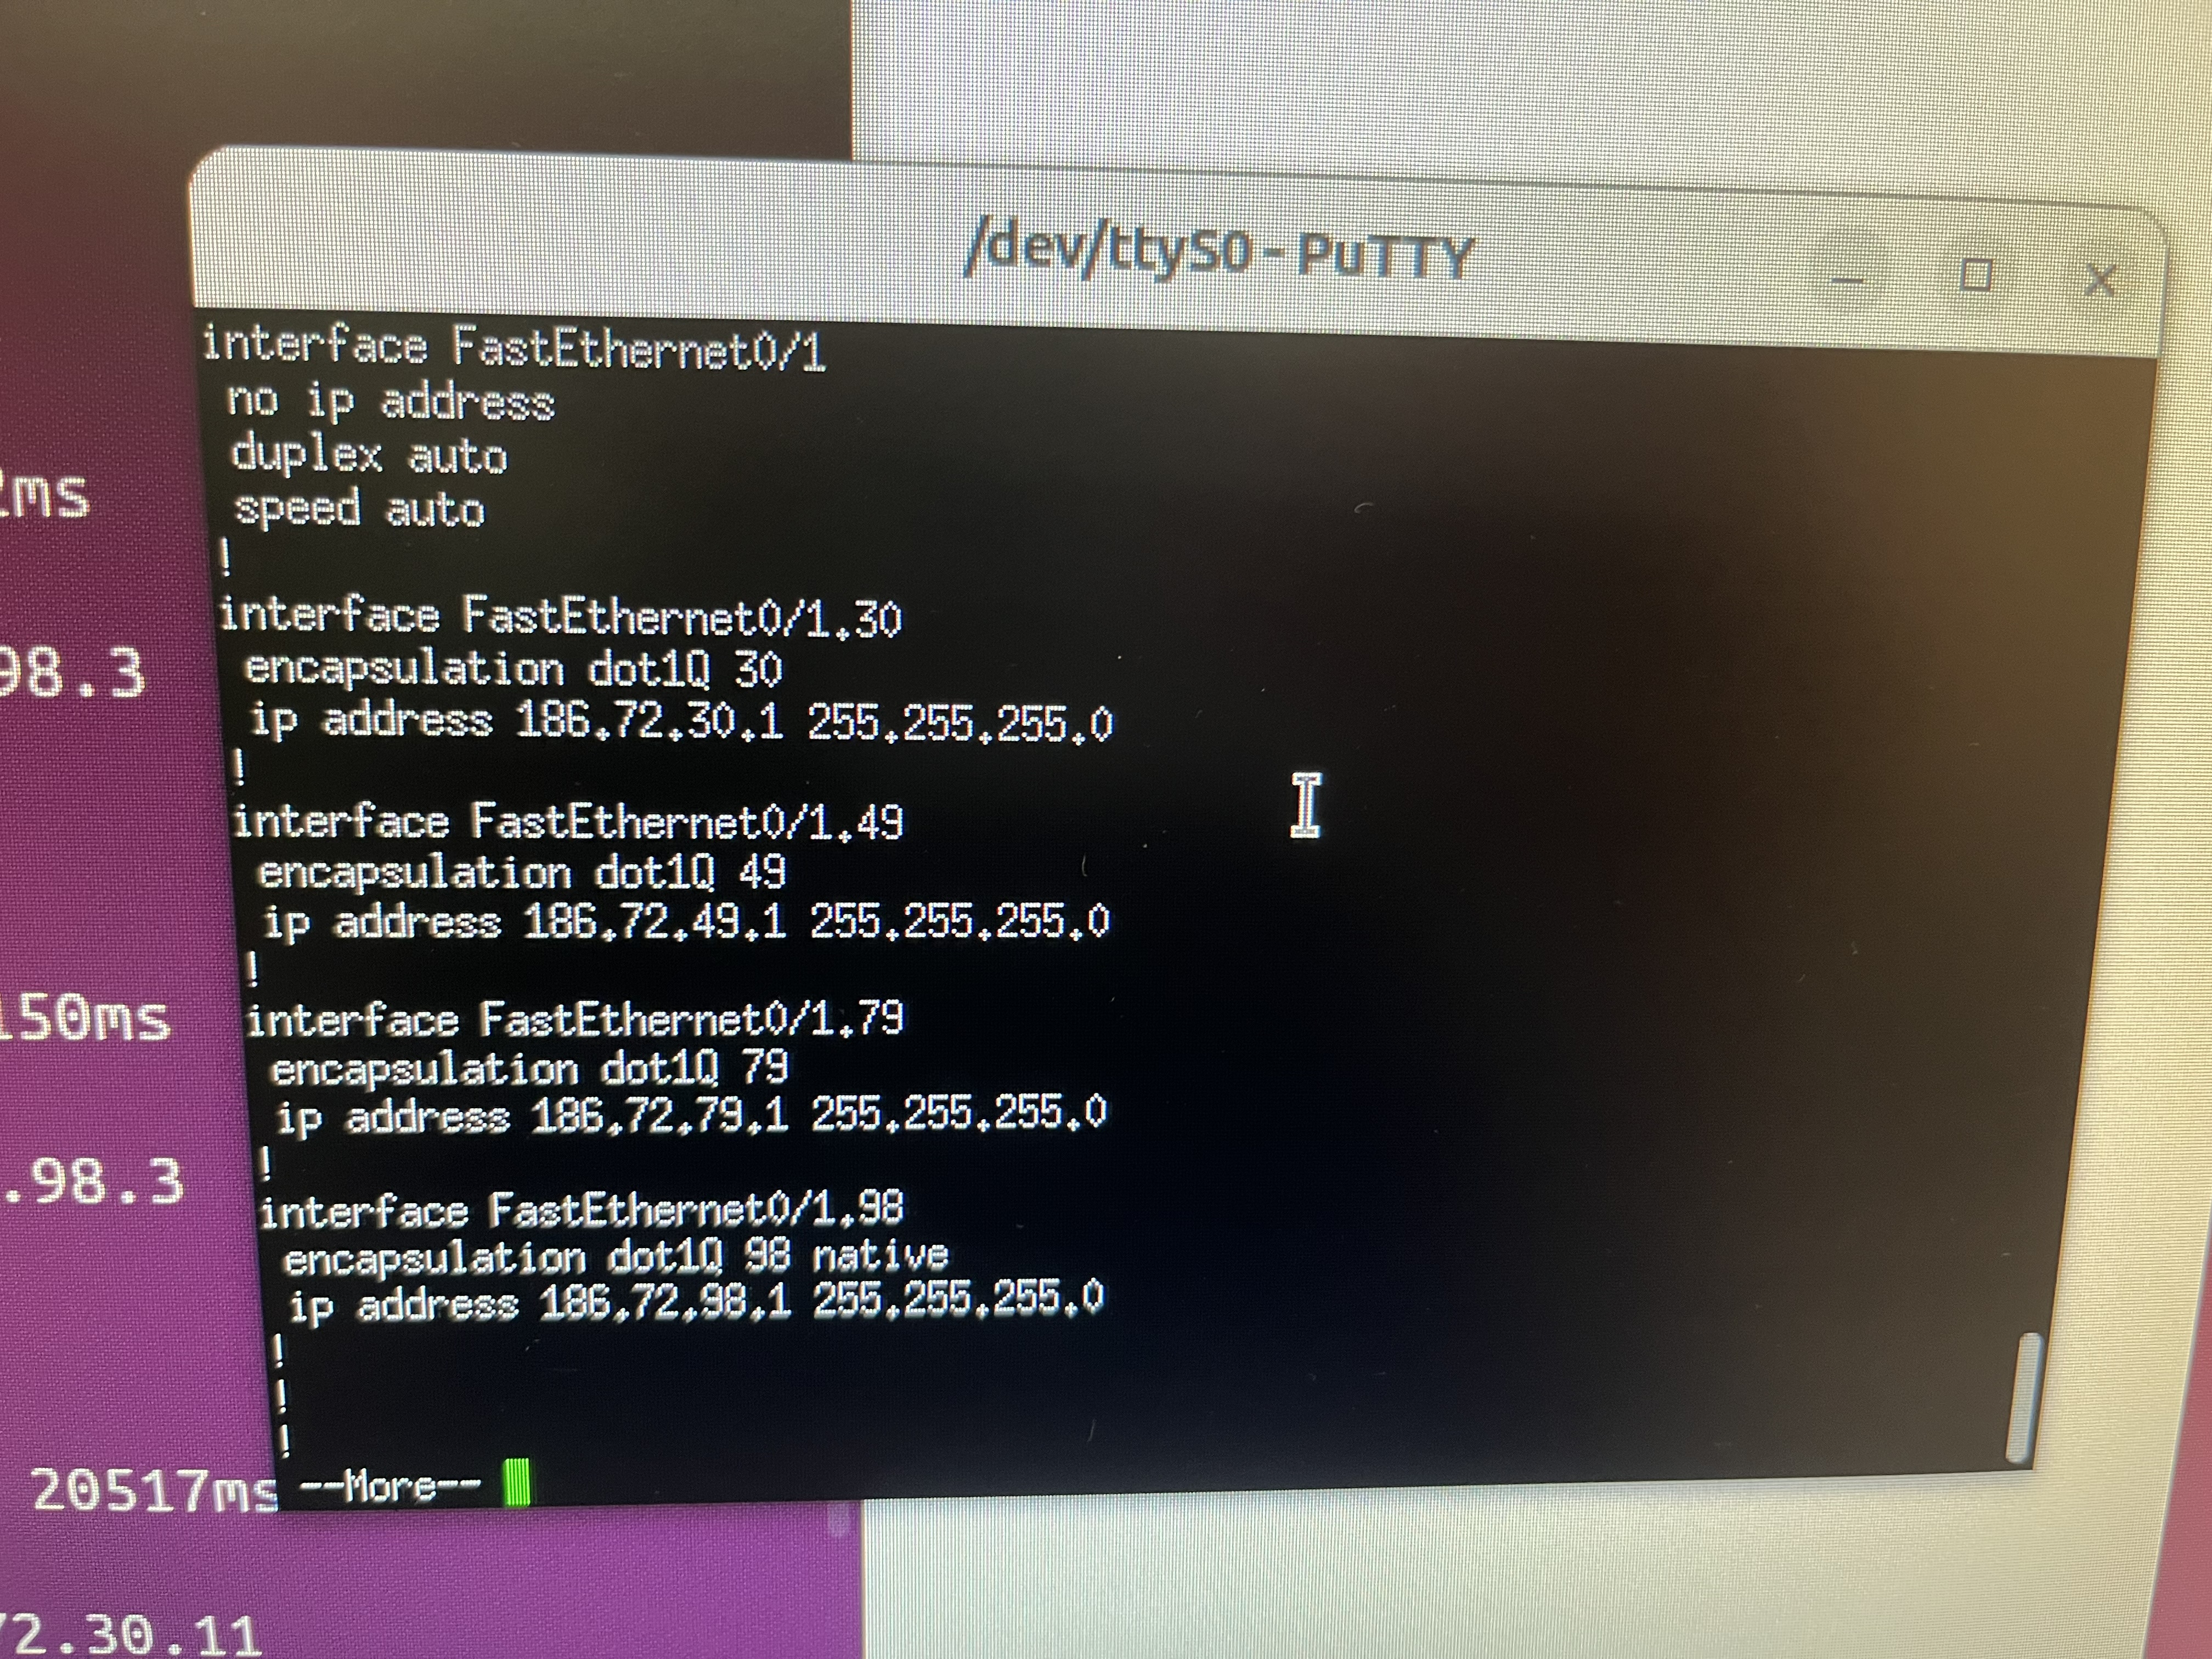
\includegraphics[width=0.8\textwidth]{practfis3.jpg}
  \caption{Evidencia de realización de práctica en equipo físico}\label{fig:practfis3}
\end{figure}

\begin{figure}[H]
  \centering
  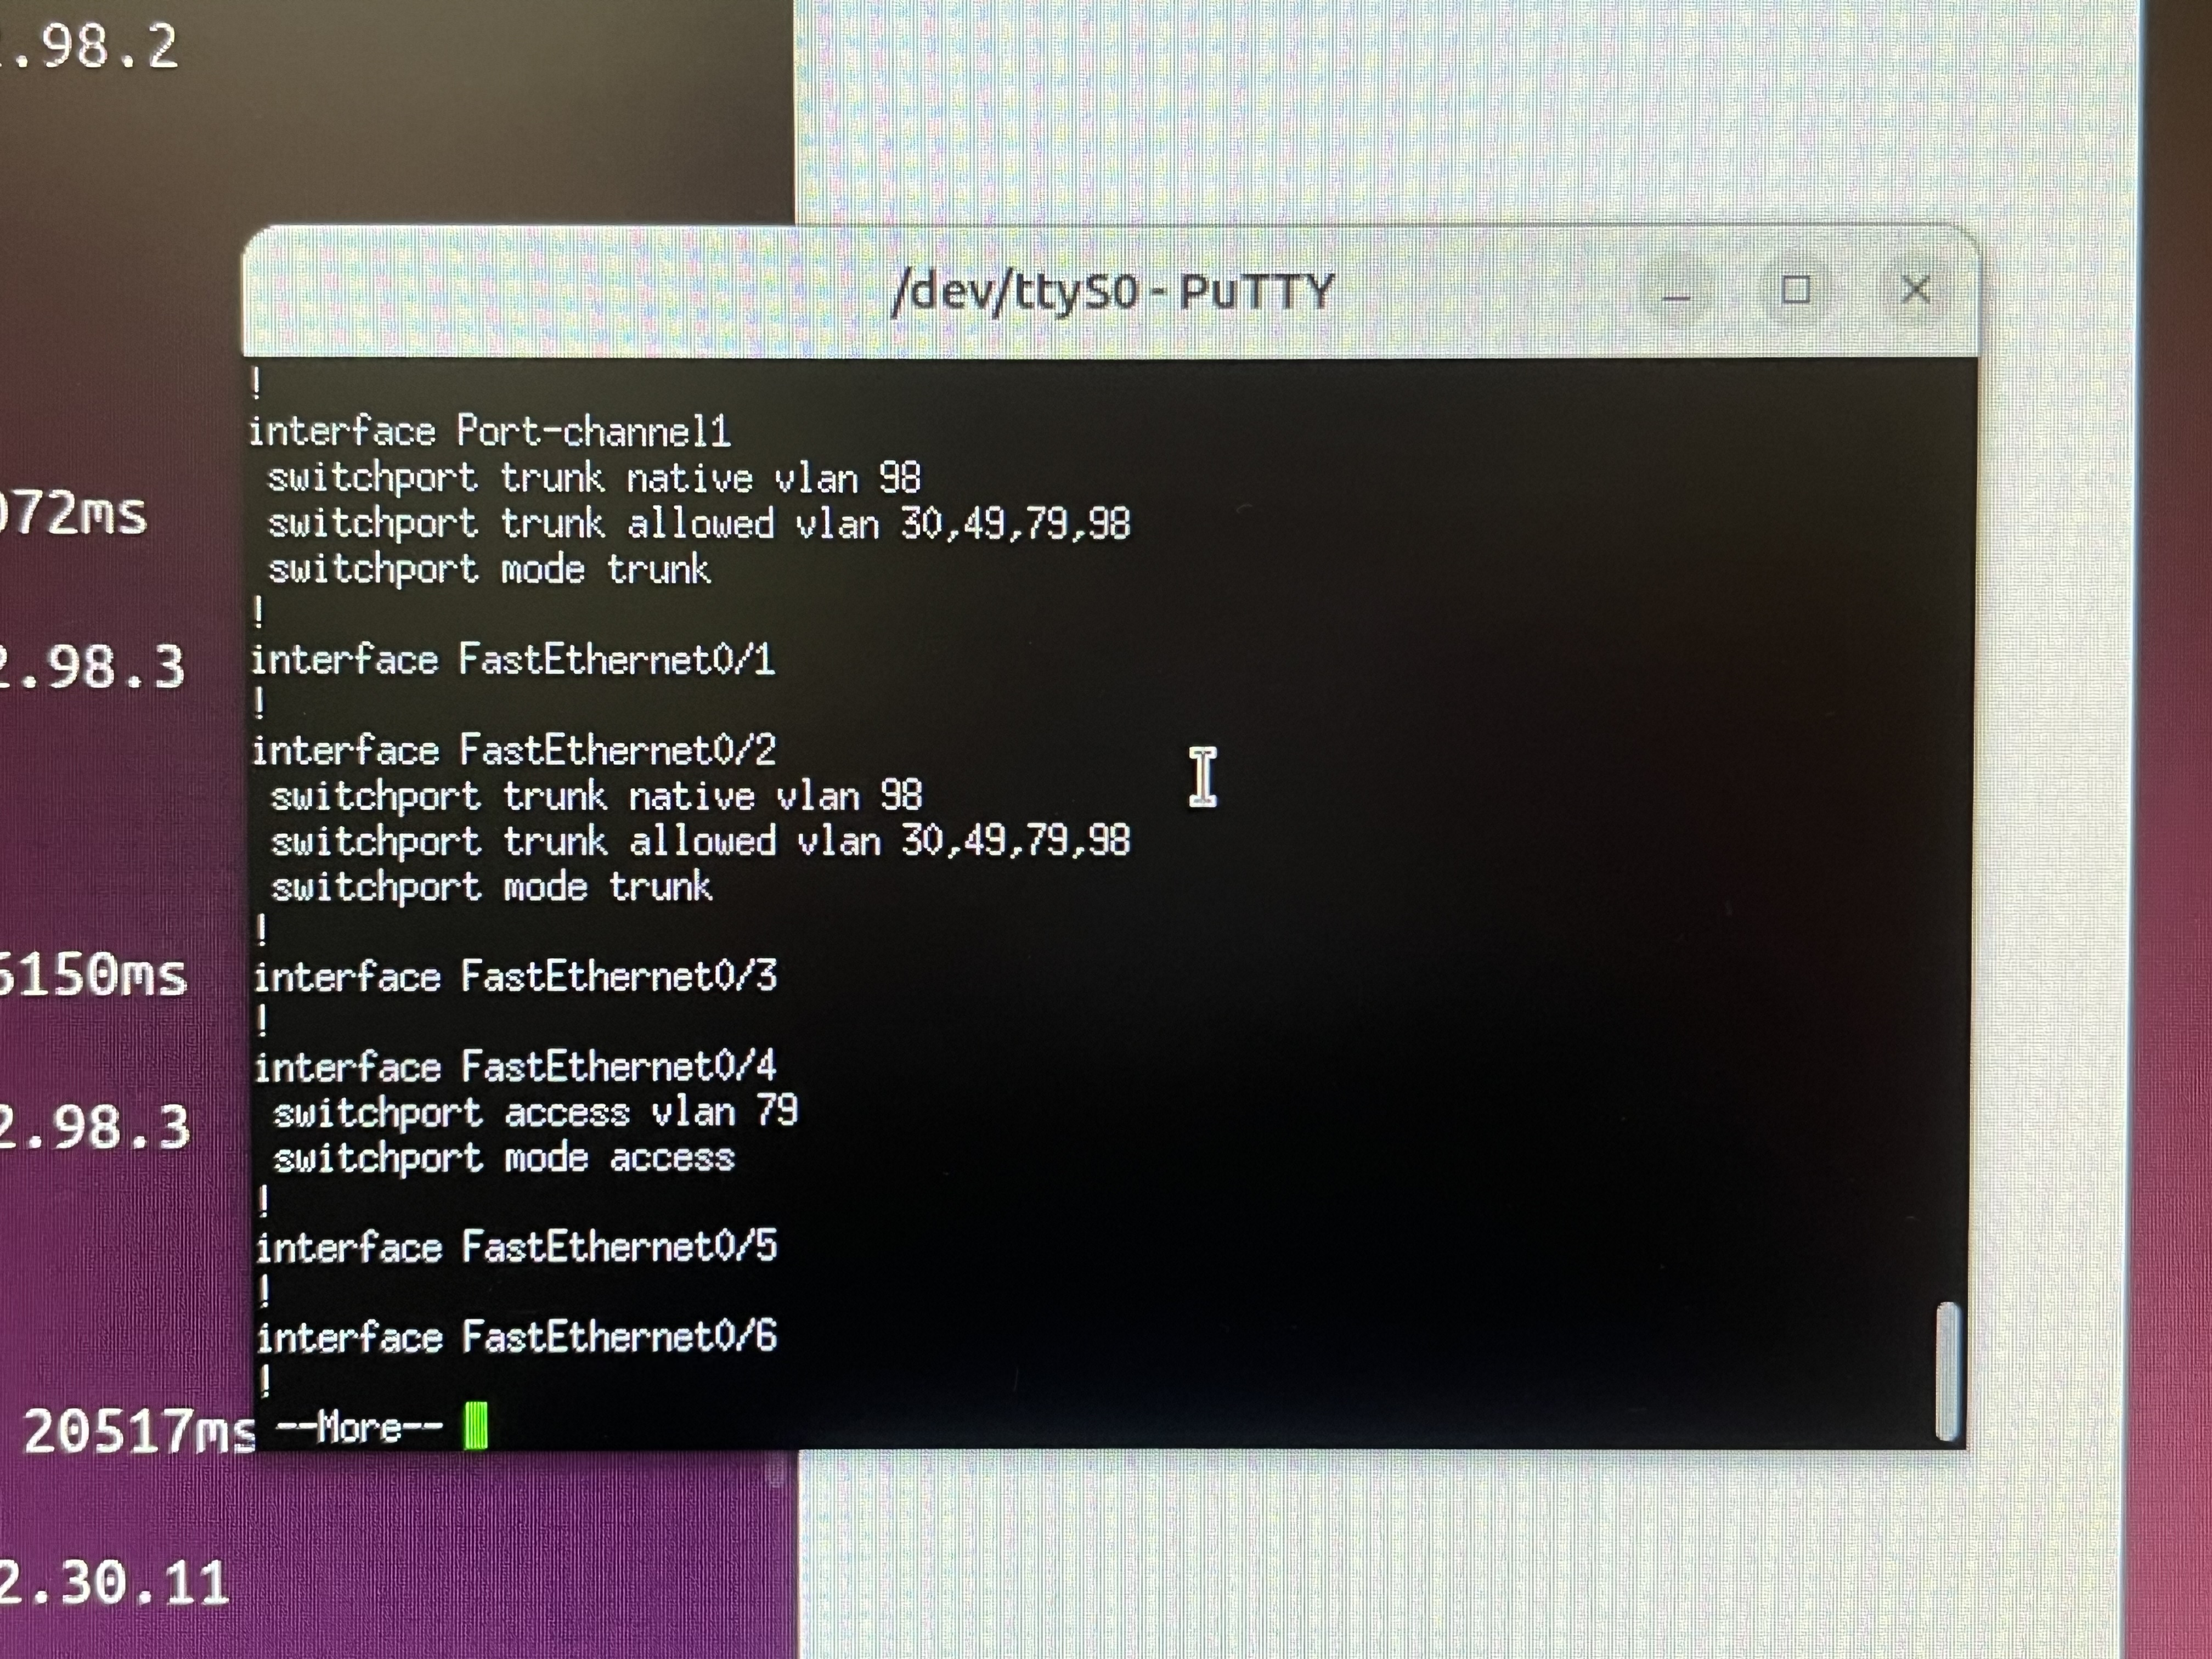
\includegraphics[width=0.8\textwidth]{practfis4.jpg}
  \caption{Evidencia de realización de práctica en equipo físico}\label{fig:practfis4}
\end{figure}

\begin{figure}[H]
  \centering
  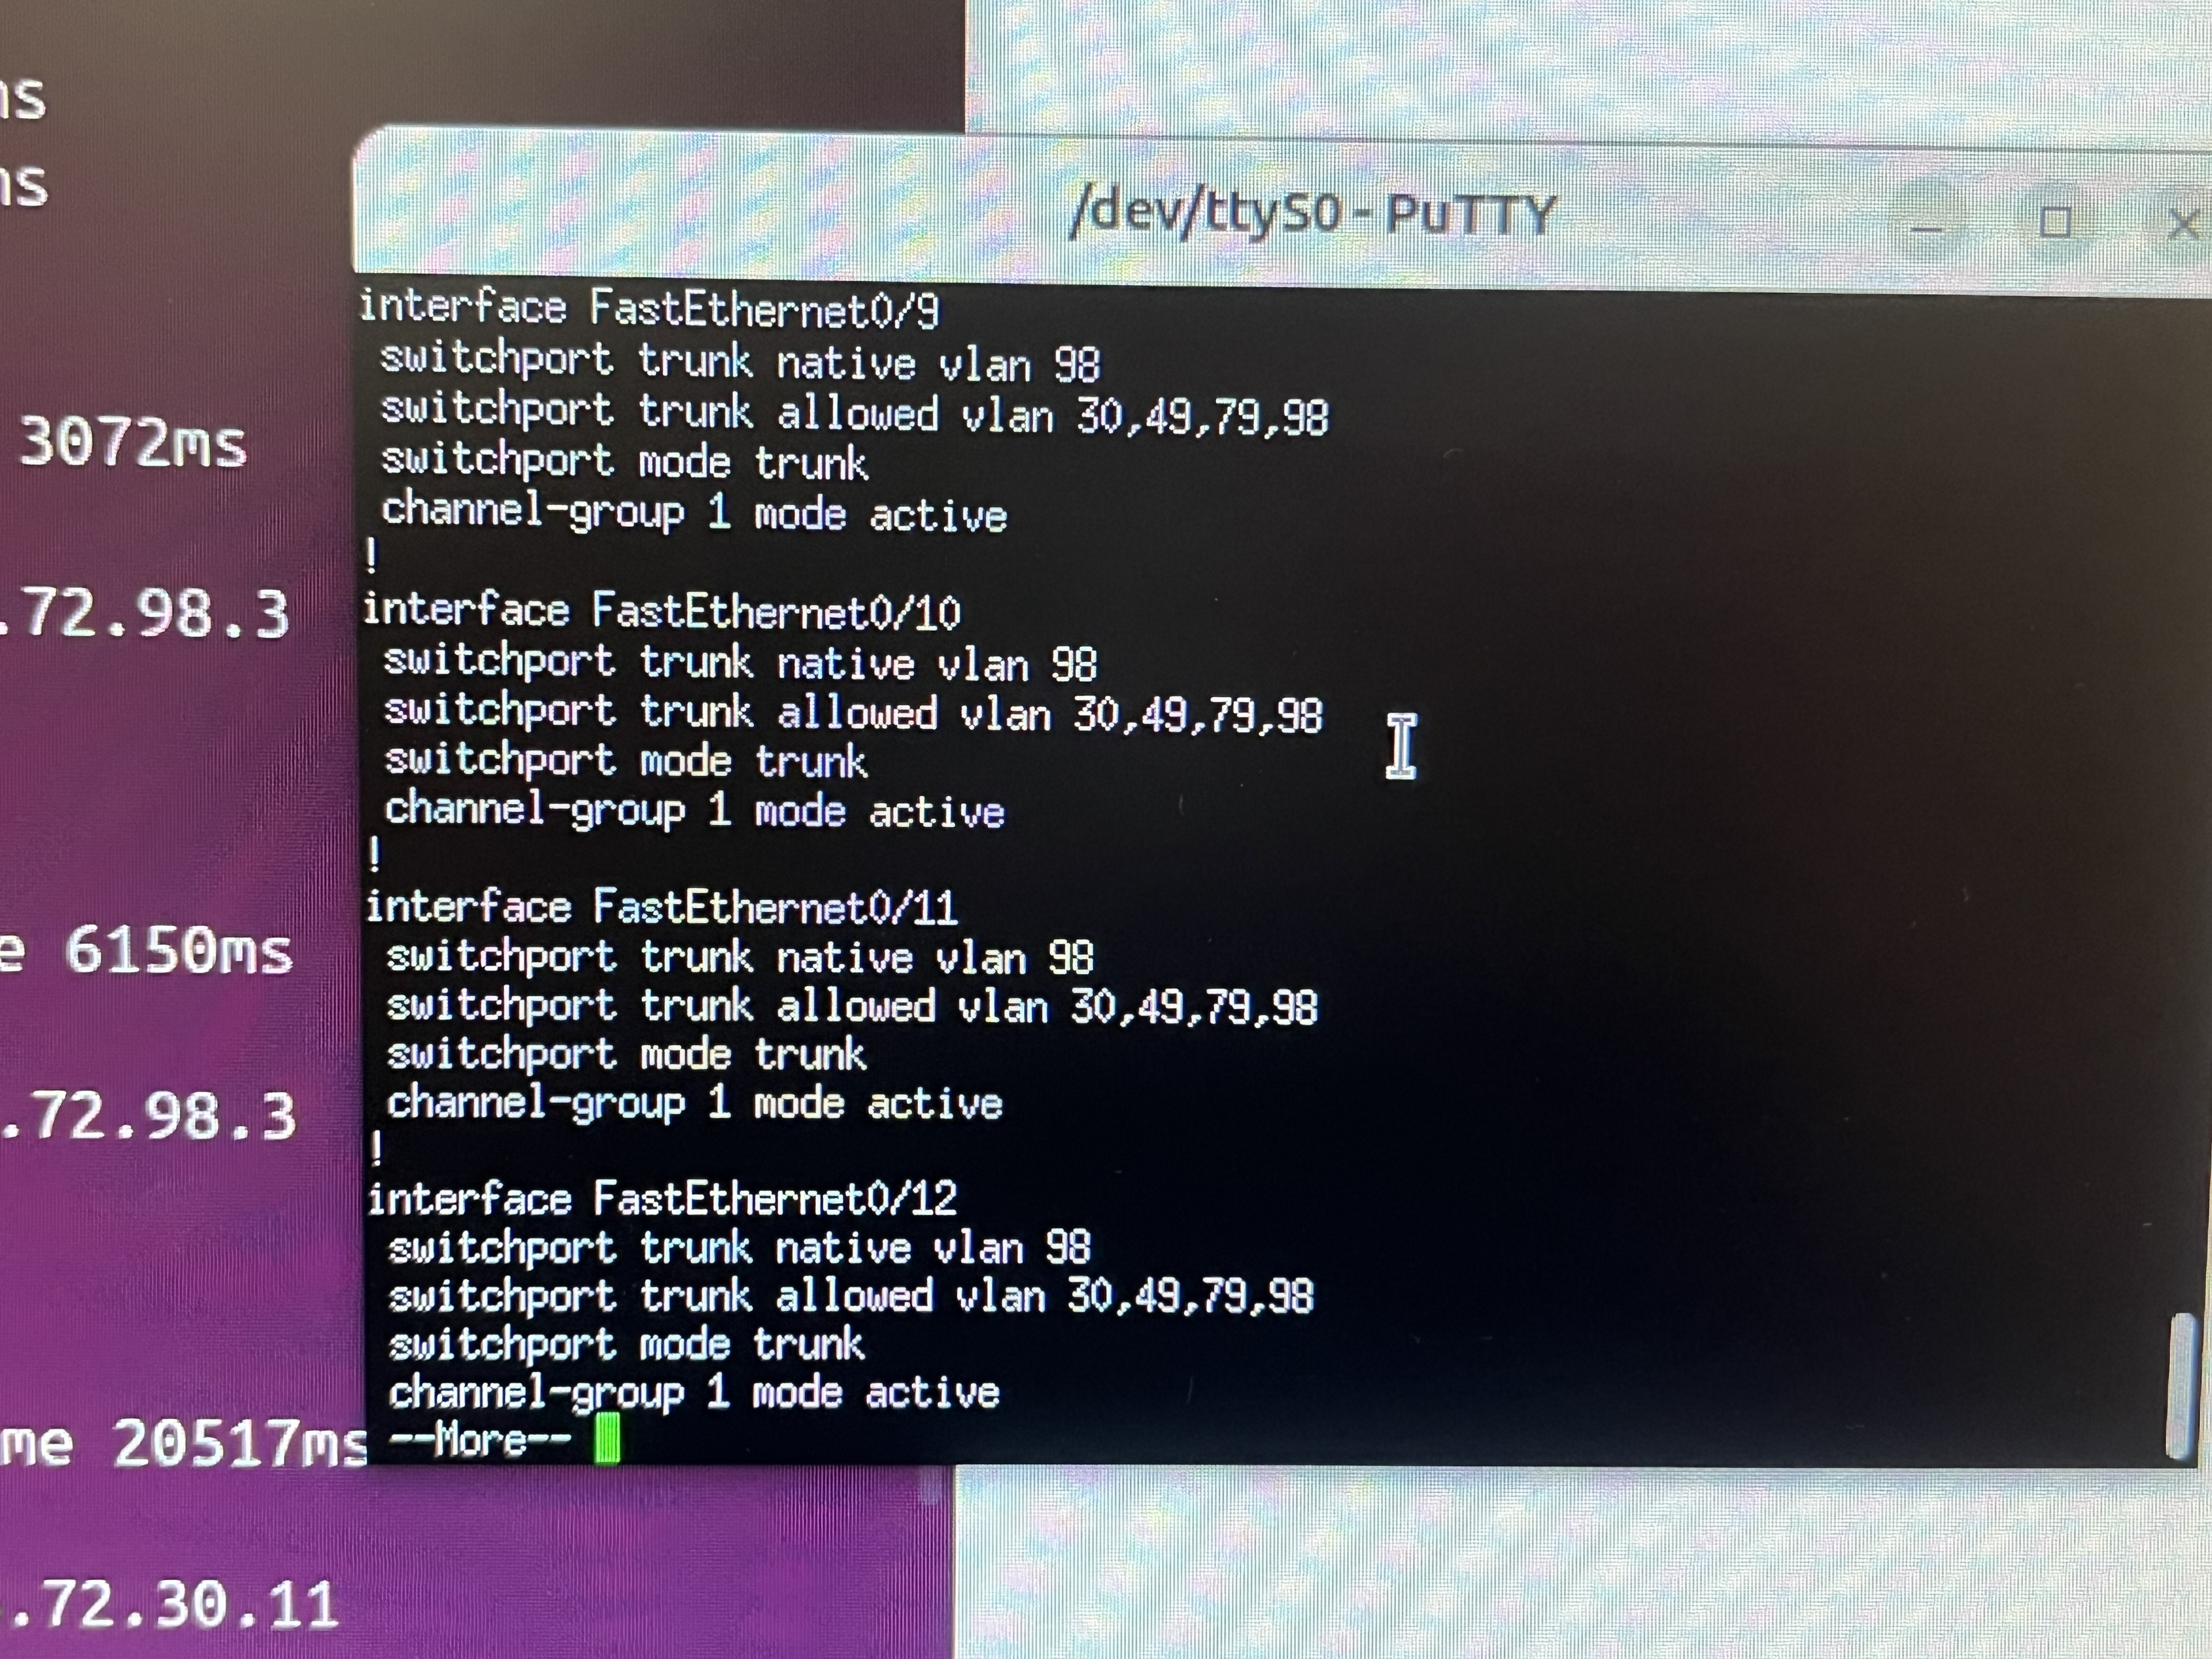
\includegraphics[width=0.8\textwidth]{practfis5.jpg}
  \caption{Evidencia de realización de práctica en equipo físico}\label{fig:practfis5}
\end{figure}

\begin{figure}[H]
  \centering
  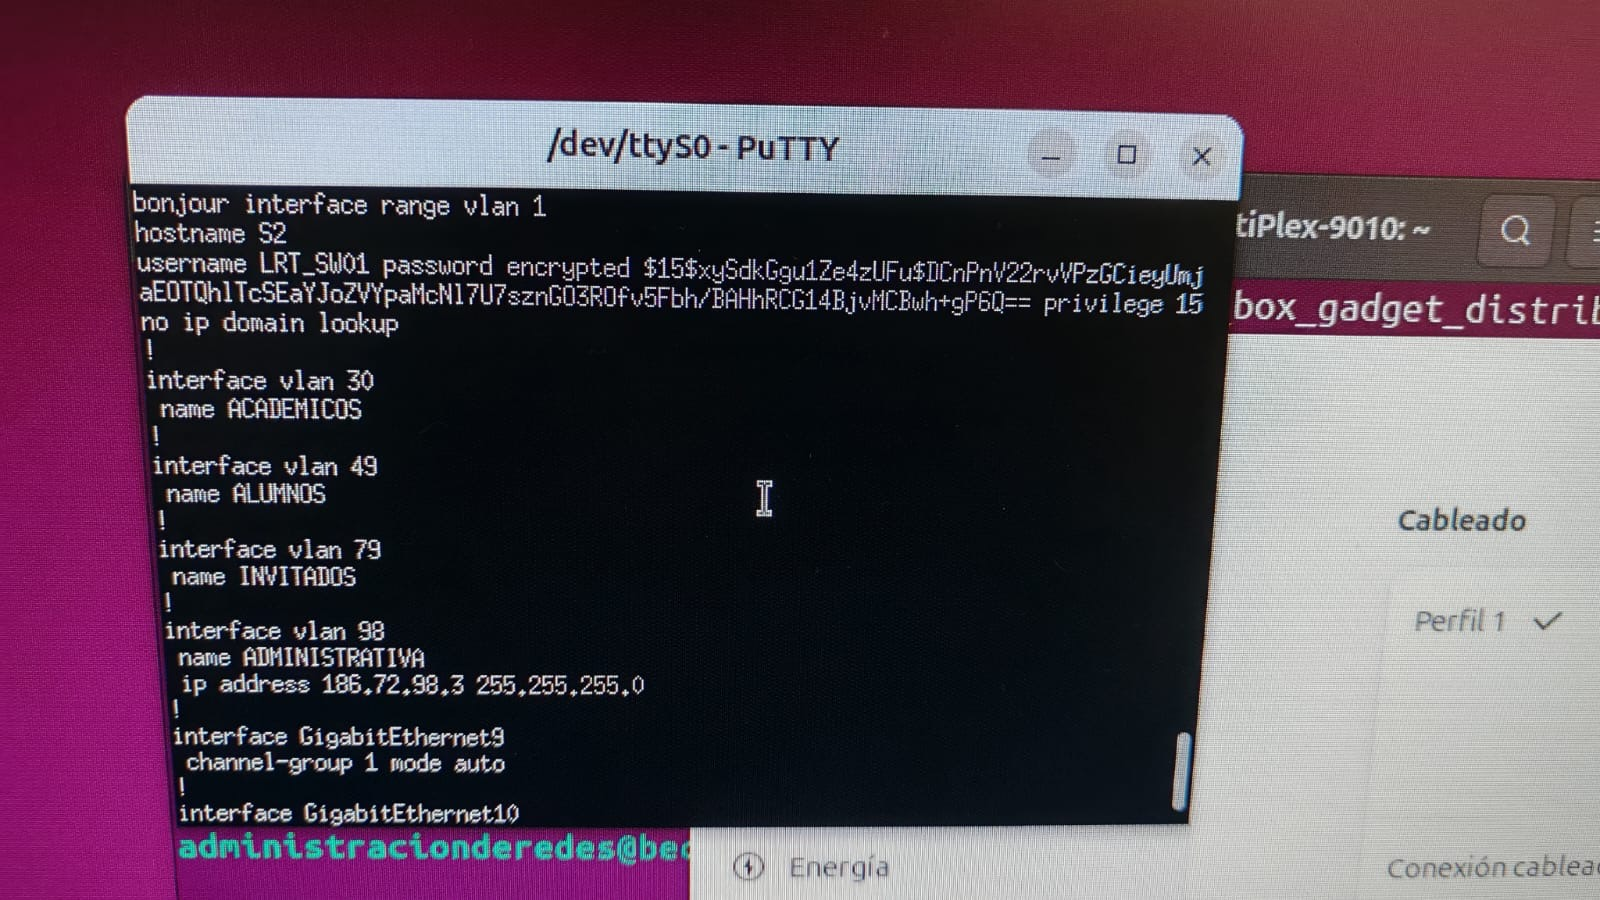
\includegraphics[width=0.8\textwidth]{practfis6.jpeg}
  \caption{Evidencia de realización de práctica en equipo físico}\label{fig:practfis6}
\end{figure}

\begin{figure}[H]
  \centering
  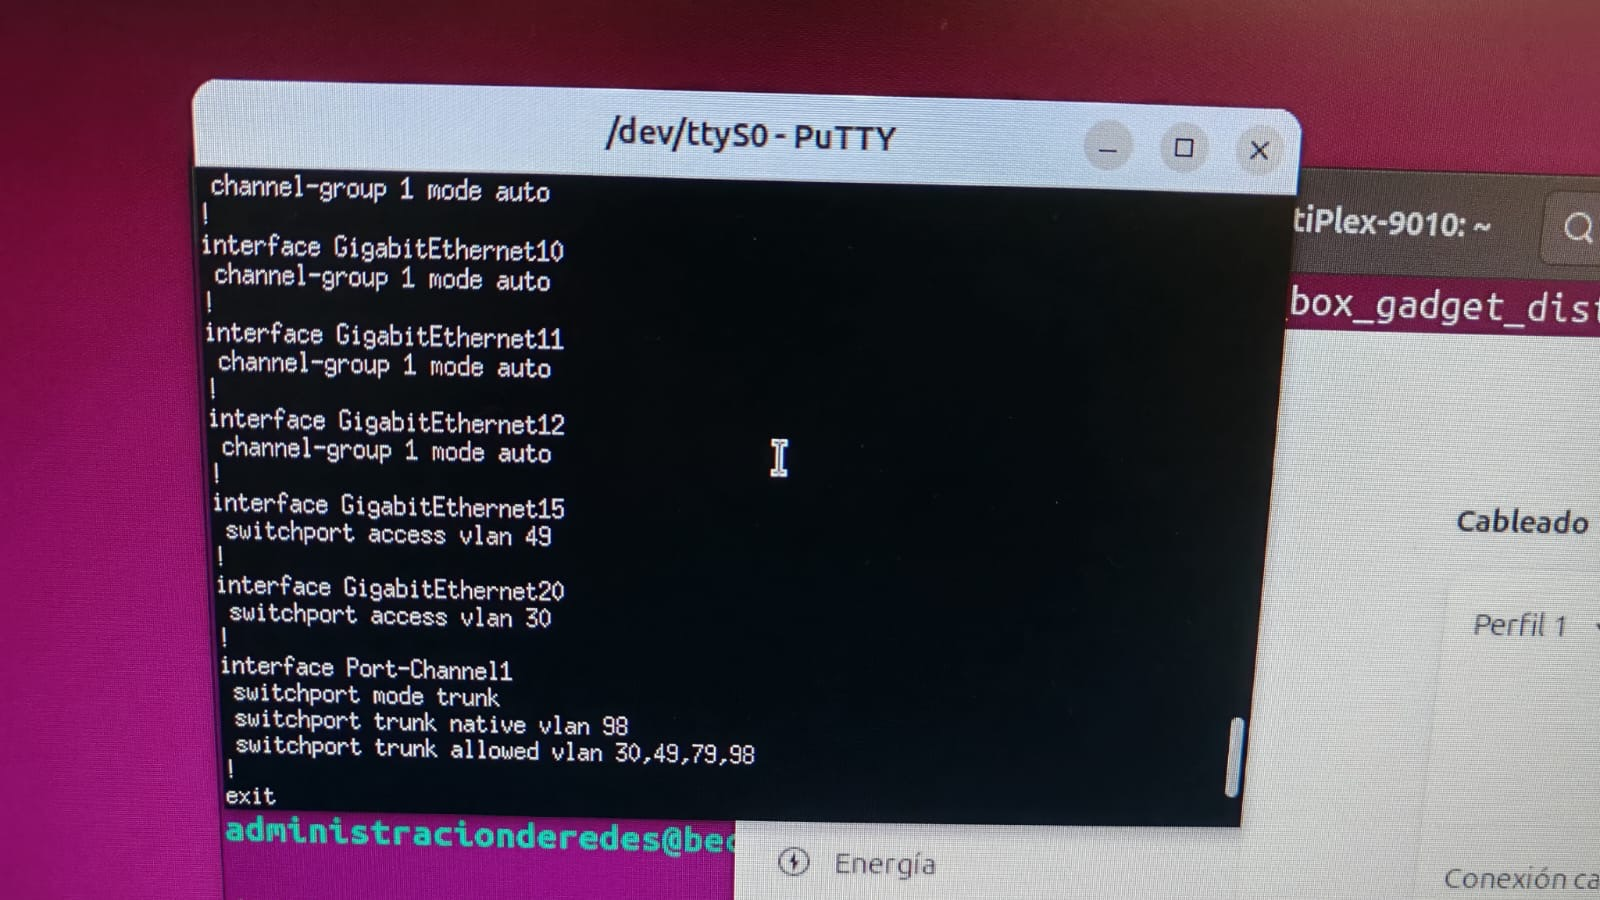
\includegraphics[width=0.8\textwidth]{practfis7.jpeg}
  \caption{Evidencia de realización de práctica en equipo físico}\label{fig:practfis7}
\end{figure}




\section{Pruebas de conectividad}
Podemos observar en la imagen, las pruebas de conectividad solicitadas en la especificación de la práctica en el simulador 
de Packet Tracer.

\begin{figure}[H]
  \centering
  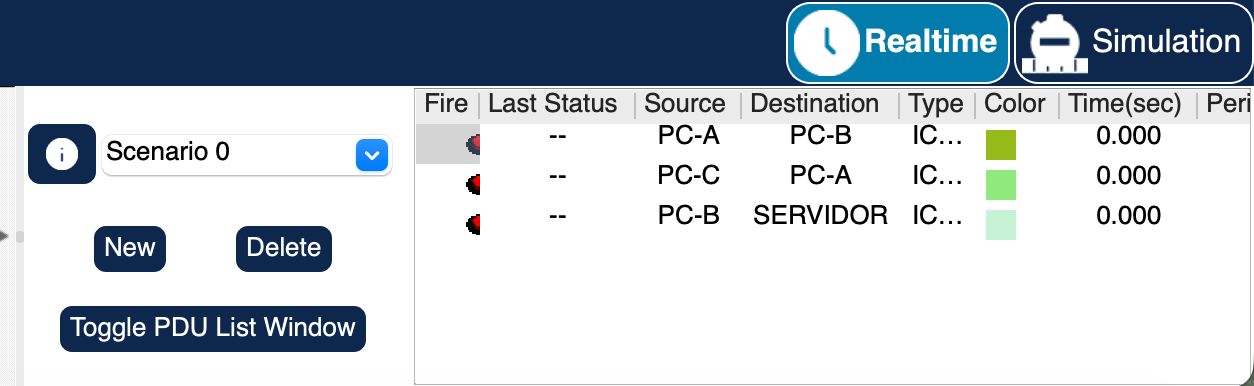
\includegraphics[width=0.8\textwidth]{pings.png}
  \caption{Pruebas de conectividad Packet Tracer}\label{fig:pings}
\end{figure}




\end{document}
